\documentclass{whiteboard}
\begin{document}
\begin{frame}[plain,t]
\bbcover{OBI 2012 - Nível 1: Fase 1}{Consecutivos}{Prof. Edson Alves}{Faculdade UnB Gama}

\end{frame}
\begin{frame}[plain,t]
\vspace*{\fill}

\bbtext{Num sorteio que distribui prêmios, um participante inicialmente sorteia um inteiro $N$ e depois $N$ valores. O
número de pontos do participante é o tamanho da maior sequência de valores consecutivos iguais. Por exemplo,
suponhamos que um participante sorteia $N = 11$ e, nesta ordem, os valores}

\vspace{0.1in}
\bbtext{$$
30, 30, 30, 30, 40, 40, 40, 40, 40, 30, 30
$$}

\vspace{0.1in}

\bbtext{Então, o participante ganha 5 pontos, correspondentes aos 5 valores 40 consecutivos. Note que o participante
sorteou 6 valores iguais a 30, mas nem todos são consecutivos.}

\vspace{0.2in}

\bbtext{Sua tarefa é ajudar a organização do evento, escrevendo um programa que determina o número de pontos de
um participante.}

\vspace*{\fill}
\end{frame}
\begin{frame}[plain,t]
\vspace*{\fill}

\bbbold{Entrada}

\vspace{0.2in}

\bbtext{A primeira linha da entrada contém um inteiro $N$, o número de valores sorteados. A segunda linha contém $N$
valores, $V_1, V_2, \ldots, V_N$, na ordem de sorteio, separados por um espaço em branco.}

\vspace{0.2in}

\bbbold{Saída}

\vspace{0.2in}

\bbtext{Seu programa deve imprimir apenas uma linha, contendo apenas um inteiro, indicando o número de pontos do
participante.}

\vspace{0.2in}

\bbbold{Restrições}
\vspace{-0.1in}

\bbtext{
\begin{itemize}
\item $1\leq N\leq 10^4$
\item $-2^{31}\leq V_i\leq 2^{31} - 1$\bbtext{, para} $i = 1, 2, \ldots, N$
\end{itemize}
}
\vspace*{\fill}
\end{frame}
\begin{frame}[plain,t]
\begin{tikzpicture}
\node[draw,opacity=0] at (0, 0) {x};
\node[draw,opacity=0] at (14, 8) {x};

	\node[anchor=west] (header) at (0, 7.0) { \bbbold{Exemplo de entrada e saída} };

\end{tikzpicture}
\end{frame}
\begin{frame}[plain,t]
\begin{tikzpicture}
\node[draw,opacity=0] at (0, 0) {x};
\node[draw,opacity=0] at (14, 8) {x};

	\node[anchor=west] (header) at (0, 7.0) { \bbbold{Exemplo de entrada e saída} };


	\node[anchor=west] (line1) at (1.0, 6.0) { \bbtext{\texttt{11} } };

\end{tikzpicture}
\end{frame}
\begin{frame}[plain,t]
\begin{tikzpicture}
\node[draw,opacity=0] at (0, 0) {x};
\node[draw,opacity=0] at (14, 8) {x};

	\node[anchor=west] (header) at (0, 7.0) { \bbbold{Exemplo de entrada e saída} };


	\node[anchor=west] (line1) at (1.0, 6.0) { \bbtext{\texttt{11} } };


	\draw[->,color=BBViolet] (1.35, 5.0) to  (1.35, 5.75);

	\node[anchor=west] (r) at (0.5, 4.75) { \footnotesize \bbcomment{\# de valores sorteados} };

\end{tikzpicture}
\end{frame}
\begin{frame}[plain,t]
\begin{tikzpicture}
\node[draw,opacity=0] at (0, 0) {x};
\node[draw,opacity=0] at (14, 8) {x};

	\node[anchor=west] (header) at (0, 7.0) { \bbbold{Exemplo de entrada e saída} };


	\node[anchor=west] (line1) at (1.0, 6.0) { \bbtext{\texttt{11} } };





	\node[anchor=west] (line2) at (1.0, 5.5) { \bbtext{\texttt{30 30 30 40 40 40 40 40 30 30 30}} };

\end{tikzpicture}
\end{frame}
\begin{frame}[plain,t]
\begin{tikzpicture}
\node[draw,opacity=0] at (0, 0) {x};
\node[draw,opacity=0] at (14, 8) {x};

	\node[anchor=west] (header) at (0, 7.0) { \bbbold{Exemplo de entrada e saída} };


	\node[anchor=west] (line1) at (1.0, 6.0) { \bbtext{\texttt{11} } };


	\draw[->,color=BBViolet] (4.35, 5.0) to  (4.35, 3.75);

	\node[anchor=west] (r) at (3.25, 3.25) { \footnotesize \bbcomment{Números sorteados} };


	\node[anchor=west] (line2) at (1.0, 5.5) { \bbtext{\texttt{30 30 30 40 40 40 40 40 30 30 30}} };





\end{tikzpicture}
\end{frame}
\begin{frame}[plain,t]
\begin{tikzpicture}
\node[draw,opacity=0] at (0, 0) {x};
\node[draw,opacity=0] at (14, 8) {x};

	\node[anchor=west] (header) at (0, 7.0) { \bbbold{Exemplo de entrada e saída} };


	\node[anchor=west] (line1) at (1.0, 6.0) { \bbtext{\texttt{11} } };





	\node[anchor=west] (line2) at (1.0, 5.5) { \bbtext{\texttt{30 30 30 40 40 40 40 40 30 30 30}} };







	\node[draw,very thick,circle] (node1) at (2.0, 3.0) { \bbtext{\texttt{30}} };

	\node[draw,very thick,circle] (node2) at (3.0, 3.0) { \bbtext{\texttt{30}} };

	\node[draw,very thick,circle] (node3) at (4.0, 3.0) { \bbtext{\texttt{30}} };

	\node[draw,very thick,circle] (node4) at (5.0, 3.0) { \bbtext{\texttt{40}} };

	\node[draw,very thick,circle] (node5) at (6.0, 3.0) { \bbtext{\texttt{40}} };

	\node[draw,very thick,circle] (node6) at (7.0, 3.0) { \bbtext{\texttt{40}} };

	\node[draw,very thick,circle] (node7) at (8.0, 3.0) { \bbtext{\texttt{40}} };

	\node[draw,very thick,circle] (node8) at (9.0, 3.0) { \bbtext{\texttt{40}} };

	\node[draw,very thick,circle] (node9) at (10.0, 3.0) { \bbtext{\texttt{30}} };

	\node[draw,very thick,circle] (node10) at (11.0, 3.0) { \bbtext{\texttt{30}} };

	\node[draw,very thick,circle] (node11) at (12.0, 3.0) { \bbtext{\texttt{30}} };

\end{tikzpicture}
\end{frame}
\begin{frame}[plain,t]
\begin{tikzpicture}
\node[draw,opacity=0] at (0, 0) {x};
\node[draw,opacity=0] at (14, 8) {x};

	\node[anchor=west] (header) at (0, 7.0) { \bbbold{Exemplo de entrada e saída} };


	\node[anchor=west] (line1) at (1.0, 6.0) { \bbtext{\texttt{11} } };





	\node[anchor=west] (line2) at (1.0, 5.5) { \bbtext{\texttt{30 30 30 40 40 40 40 40 30 30 30}} };







	\node[draw,very thick,circle,fill=BBGreen] (node1) at (2.0, 3.0) { \bbtext{\texttt{30}} };

	\node[draw,very thick,circle,fill=BBGreen] (node2) at (3.0, 3.0) { \bbtext{\texttt{30}} };

	\node[draw,very thick,circle,fill=BBGreen] (node3) at (4.0, 3.0) { \bbtext{\texttt{30}} };

	\node[draw,very thick,circle] (node4) at (5.0, 3.0) { \bbtext{\texttt{40}} };

	\node[draw,very thick,circle] (node5) at (6.0, 3.0) { \bbtext{\texttt{40}} };

	\node[draw,very thick,circle] (node6) at (7.0, 3.0) { \bbtext{\texttt{40}} };

	\node[draw,very thick,circle] (node7) at (8.0, 3.0) { \bbtext{\texttt{40}} };

	\node[draw,very thick,circle] (node8) at (9.0, 3.0) { \bbtext{\texttt{40}} };

	\node[draw,very thick,circle] (node9) at (10.0, 3.0) { \bbtext{\texttt{30}} };

	\node[draw,very thick,circle] (node10) at (11.0, 3.0) { \bbtext{\texttt{30}} };

	\node[draw,very thick,circle] (node11) at (12.0, 3.0) { \bbtext{\texttt{30}} };



\end{tikzpicture}
\end{frame}
\begin{frame}[plain,t]
\begin{tikzpicture}
\node[draw,opacity=0] at (0, 0) {x};
\node[draw,opacity=0] at (14, 8) {x};

	\node[anchor=west] (header) at (0, 7.0) { \bbbold{Exemplo de entrada e saída} };


	\node[anchor=west] (line1) at (1.0, 6.0) { \bbtext{\texttt{11} } };





	\node[anchor=west] (line2) at (1.0, 5.5) { \bbtext{\texttt{30 30 30 40 40 40 40 40 30 30 30}} };







	\node[draw,very thick,circle,fill=BBWhite] (node1) at (2.0, 3.0) { \bbtext{\texttt{30}} };

	\node[draw,very thick,circle,fill=BBWhite] (node2) at (3.0, 3.0) { \bbtext{\texttt{30}} };

	\node[draw,very thick,circle,fill=BBWhite] (node3) at (4.0, 3.0) { \bbtext{\texttt{30}} };

	\node[draw,very thick,circle,fill=BBCyan] (node4) at (5.0, 3.0) { \bbtext{\texttt{40}} };

	\node[draw,very thick,circle,fill=BBCyan] (node5) at (6.0, 3.0) { \bbtext{\texttt{40}} };

	\node[draw,very thick,circle,fill=BBCyan] (node6) at (7.0, 3.0) { \bbtext{\texttt{40}} };

	\node[draw,very thick,circle,fill=BBCyan] (node7) at (8.0, 3.0) { \bbtext{\texttt{40}} };

	\node[draw,very thick,circle,fill=BBCyan] (node8) at (9.0, 3.0) { \bbtext{\texttt{40}} };

	\node[draw,very thick,circle] (node9) at (10.0, 3.0) { \bbtext{\texttt{30}} };

	\node[draw,very thick,circle] (node10) at (11.0, 3.0) { \bbtext{\texttt{30}} };

	\node[draw,very thick,circle] (node11) at (12.0, 3.0) { \bbtext{\texttt{30}} };






\end{tikzpicture}
\end{frame}
\begin{frame}[plain,t]
\begin{tikzpicture}
\node[draw,opacity=0] at (0, 0) {x};
\node[draw,opacity=0] at (14, 8) {x};

	\node[anchor=west] (header) at (0, 7.0) { \bbbold{Exemplo de entrada e saída} };


	\node[anchor=west] (line1) at (1.0, 6.0) { \bbtext{\texttt{11} } };





	\node[anchor=west] (line2) at (1.0, 5.5) { \bbtext{\texttt{30 30 30 40 40 40 40 40 30 30 30}} };







	\node[draw,very thick,circle,fill=BBWhite] (node1) at (2.0, 3.0) { \bbtext{\texttt{30}} };

	\node[draw,very thick,circle,fill=BBWhite] (node2) at (3.0, 3.0) { \bbtext{\texttt{30}} };

	\node[draw,very thick,circle,fill=BBWhite] (node3) at (4.0, 3.0) { \bbtext{\texttt{30}} };

	\node[draw,very thick,circle,fill=BBWhite] (node4) at (5.0, 3.0) { \bbtext{\texttt{40}} };

	\node[draw,very thick,circle,fill=BBWhite] (node5) at (6.0, 3.0) { \bbtext{\texttt{40}} };

	\node[draw,very thick,circle,fill=BBWhite] (node6) at (7.0, 3.0) { \bbtext{\texttt{40}} };

	\node[draw,very thick,circle,fill=BBWhite] (node7) at (8.0, 3.0) { \bbtext{\texttt{40}} };

	\node[draw,very thick,circle,fill=BBWhite] (node8) at (9.0, 3.0) { \bbtext{\texttt{40}} };

	\node[draw,very thick,circle,fill=BBGreen] (node9) at (10.0, 3.0) { \bbtext{\texttt{30}} };

	\node[draw,very thick,circle,fill=BBGreen] (node10) at (11.0, 3.0) { \bbtext{\texttt{30}} };

	\node[draw,very thick,circle,fill=BBGreen] (node11) at (12.0, 3.0) { \bbtext{\texttt{30}} };









\end{tikzpicture}
\end{frame}
\begin{frame}[plain,t]
\begin{tikzpicture}
\node[draw,opacity=0] at (0, 0) {x};
\node[draw,opacity=0] at (14, 8) {x};

	\node[anchor=west] (header) at (0, 7.0) { \bbbold{Exemplo de entrada e saída} };


	\node[anchor=west] (line1) at (1.0, 6.0) { \bbtext{\texttt{11} } };


	\draw[->,color=BBBlack,-latex,thick] (8.0, 5.5) to  (10.0, 5.5);

	\node[anchor=west] (r) at (10.25, 5.5) { \footnotesize \bboutput{5} };


	\node[anchor=west] (line2) at (1.0, 5.5) { \bbtext{\texttt{30 30 30 40 40 40 40 40 30 30 30}} };







	\node[draw,very thick,circle,fill=BBWhite] (node1) at (2.0, 3.0) { \bbtext{\texttt{30}} };

	\node[draw,very thick,circle,fill=BBWhite] (node2) at (3.0, 3.0) { \bbtext{\texttt{30}} };

	\node[draw,very thick,circle,fill=BBWhite] (node3) at (4.0, 3.0) { \bbtext{\texttt{30}} };

	\node[draw,very thick,circle,fill=BBWhite] (node4) at (5.0, 3.0) { \bbtext{\texttt{40}} };

	\node[draw,very thick,circle,fill=BBWhite] (node5) at (6.0, 3.0) { \bbtext{\texttt{40}} };

	\node[draw,very thick,circle,fill=BBWhite] (node6) at (7.0, 3.0) { \bbtext{\texttt{40}} };

	\node[draw,very thick,circle,fill=BBWhite] (node7) at (8.0, 3.0) { \bbtext{\texttt{40}} };

	\node[draw,very thick,circle,fill=BBWhite] (node8) at (9.0, 3.0) { \bbtext{\texttt{40}} };

	\node[draw,very thick,circle,fill=BBGreen] (node9) at (10.0, 3.0) { \bbtext{\texttt{30}} };

	\node[draw,very thick,circle,fill=BBGreen] (node10) at (11.0, 3.0) { \bbtext{\texttt{30}} };

	\node[draw,very thick,circle,fill=BBGreen] (node11) at (12.0, 3.0) { \bbtext{\texttt{30}} };














\end{tikzpicture}
\end{frame}
\begin{frame}[plain,t]
\begin{tikzpicture}
\node[draw,opacity=0] at (0, 0) {x};
\node[draw,opacity=0] at (14, 8) {x};

	\node[anchor=west] (title) at (0.0, 7.0) { \Large \bbbold{Solução} };

\end{tikzpicture}
\end{frame}
\begin{frame}[plain,t]
\begin{tikzpicture}
\node[draw,opacity=0] at (0, 0) {x};
\node[draw,opacity=0] at (14, 8) {x};

	\node[anchor=west] (title) at (0.0, 7.0) { \Large \bbbold{Solução} };


	\node[anchor=west] (a) at (1.0, 6.0) { $\star$ \bbtext{O problema consiste em identificar as sequências de números consecutivos} };

\end{tikzpicture}
\end{frame}
\begin{frame}[plain,t]
\begin{tikzpicture}
\node[draw,opacity=0] at (0, 0) {x};
\node[draw,opacity=0] at (14, 8) {x};

	\node[anchor=west] (title) at (0.0, 7.0) { \Large \bbbold{Solução} };


	\node[anchor=west] (a) at (1.0, 6.0) { $\star$ \bbtext{O problema consiste em identificar as sequências de números consecutivos} };


	\node[anchor=west] (b) at (1.0, 5.0) { $\star$ \bbtext{Uma vez identificadas, a resposta será o tamanho da maior delas} };

\end{tikzpicture}
\end{frame}
\begin{frame}[plain,t]
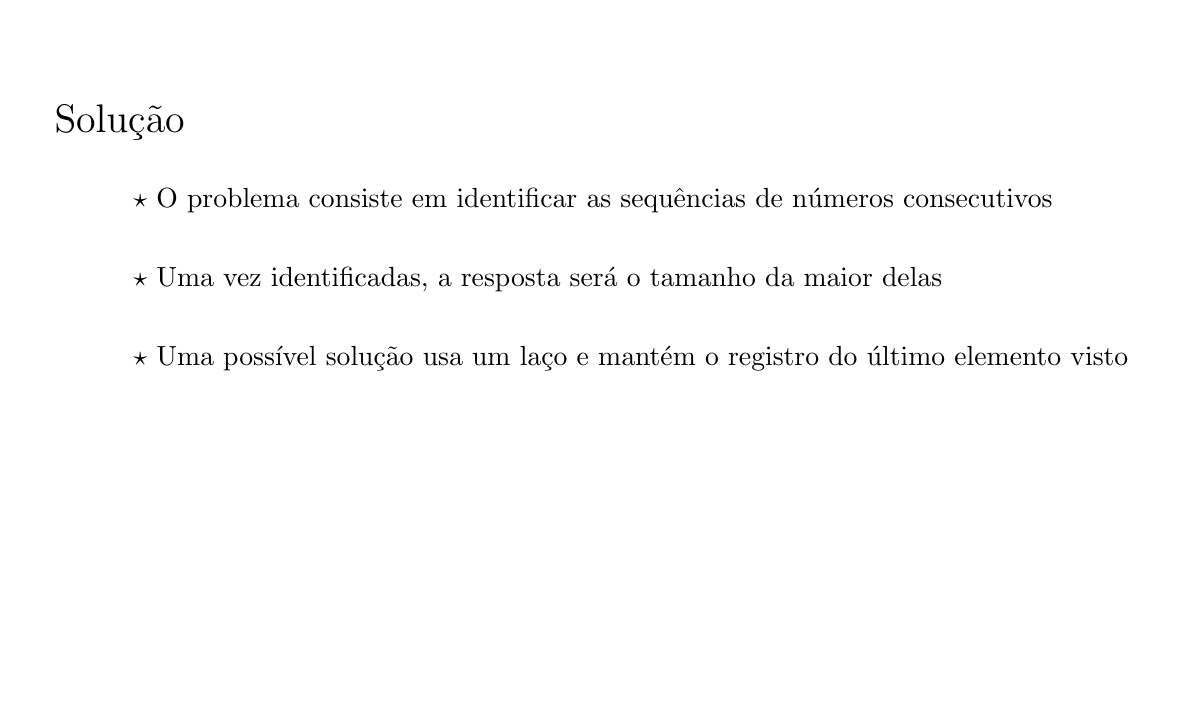
\begin{tikzpicture}
\node[draw,opacity=0] at (0, 0) {x};
\node[draw,opacity=0] at (14, 8) {x};

	\node[anchor=west] (title) at (0.0, 7.0) { \Large \bbbold{Solução} };


	\node[anchor=west] (a) at (1.0, 6.0) { $\star$ \bbtext{O problema consiste em identificar as sequências de números consecutivos} };


	\node[anchor=west] (b) at (1.0, 5.0) { $\star$ \bbtext{Uma vez identificadas, a resposta será o tamanho da maior delas} };


	\node[anchor=west] (c) at (1.0, 4.0) { $\star$ \bbtext{Uma possível solução usa um laço e mantém o registro do último elemento visto} };

\end{tikzpicture}
\end{frame}
\begin{frame}[plain,t]
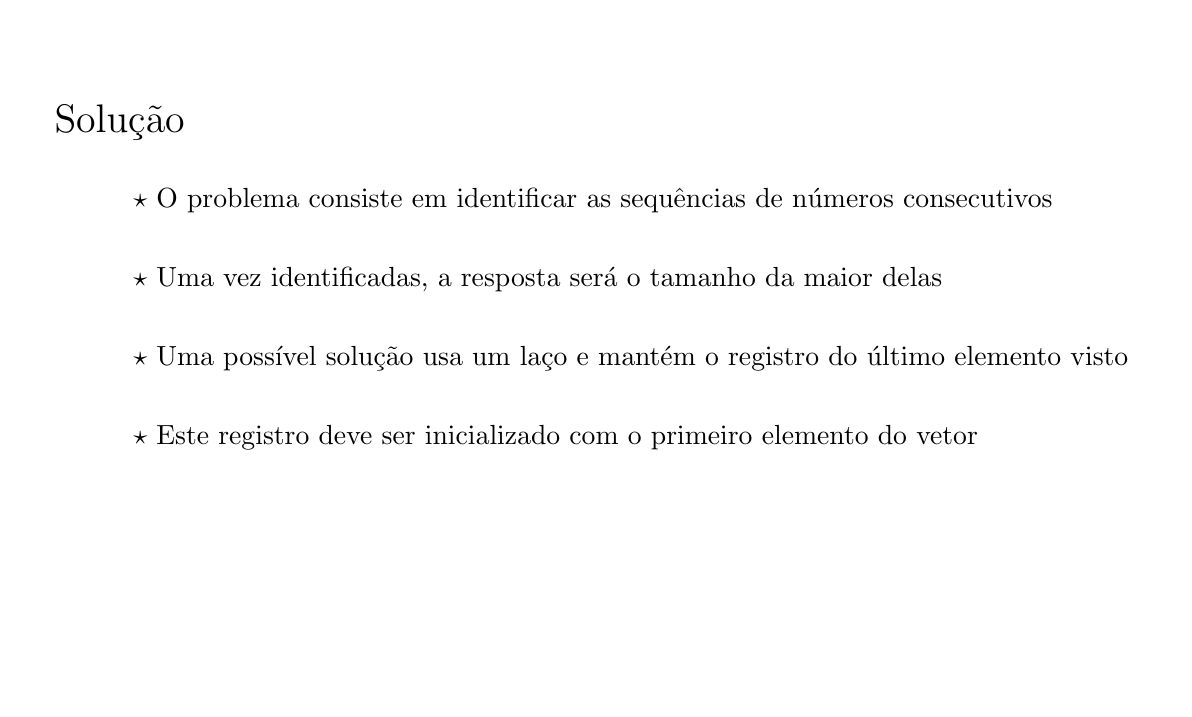
\begin{tikzpicture}
\node[draw,opacity=0] at (0, 0) {x};
\node[draw,opacity=0] at (14, 8) {x};

	\node[anchor=west] (title) at (0.0, 7.0) { \Large \bbbold{Solução} };


	\node[anchor=west] (a) at (1.0, 6.0) { $\star$ \bbtext{O problema consiste em identificar as sequências de números consecutivos} };


	\node[anchor=west] (b) at (1.0, 5.0) { $\star$ \bbtext{Uma vez identificadas, a resposta será o tamanho da maior delas} };


	\node[anchor=west] (c) at (1.0, 4.0) { $\star$ \bbtext{Uma possível solução usa um laço e mantém o registro do último elemento visto} };


	\node[anchor=west] (d) at (1.0, 3.0) { $\star$ \bbtext{Este registro deve ser inicializado com o primeiro elemento do vetor} };

\end{tikzpicture}
\end{frame}
\begin{frame}[plain,t]
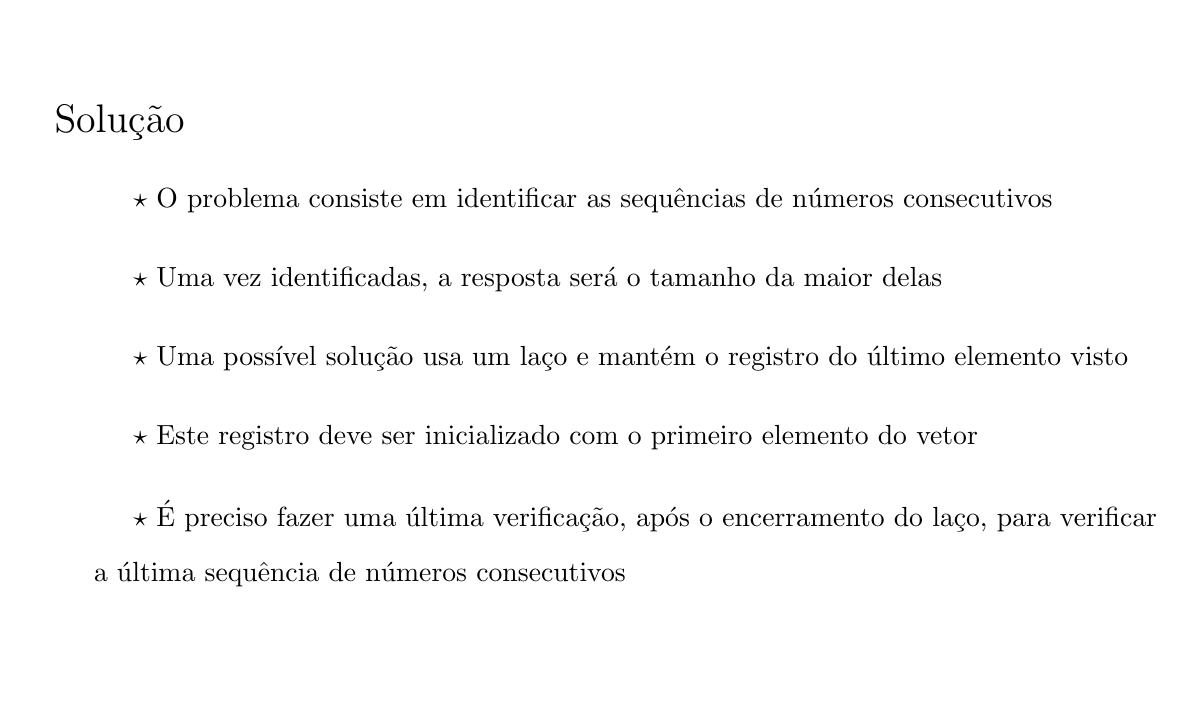
\begin{tikzpicture}
\node[draw,opacity=0] at (0, 0) {x};
\node[draw,opacity=0] at (14, 8) {x};

	\node[anchor=west] (title) at (0.0, 7.0) { \Large \bbbold{Solução} };


	\node[anchor=west] (a) at (1.0, 6.0) { $\star$ \bbtext{O problema consiste em identificar as sequências de números consecutivos} };


	\node[anchor=west] (b) at (1.0, 5.0) { $\star$ \bbtext{Uma vez identificadas, a resposta será o tamanho da maior delas} };


	\node[anchor=west] (c) at (1.0, 4.0) { $\star$ \bbtext{Uma possível solução usa um laço e mantém o registro do último elemento visto} };


	\node[anchor=west] (d) at (1.0, 3.0) { $\star$ \bbtext{Este registro deve ser inicializado com o primeiro elemento do vetor} };


	\node[anchor=west] (e) at (1.0, 2.0) { $\star$ \bbtext{É preciso fazer uma última verificação, após o encerramento do laço, para verificar} };

	\node[anchor=west] (e1) at (0.5, 1.25) { \bbtext{a última sequência de números consecutivos} };

\end{tikzpicture}
\end{frame}
\begin{frame}[plain,t]
\begin{tikzpicture}
\node[draw,opacity=0] at (0, 0) {x};
\node[draw,opacity=0] at (14, 8) {x};

	\node[anchor=west] (line1) at (1.0, 8.0) { \inputline{c}{1}{codes/solution.c} };

	\node[anchor=west] (line2) at (1.0, 7.62) { \inputline{c}{2}{codes/solution.c} };

	\node[anchor=west] (line3) at (1.0, 7.24) { \inputline{c}{3}{codes/solution.c} };

	\node[anchor=west] (line4) at (1.0, 6.86) { \inputline{c}{4}{codes/solution.c} };



















	\draw[color=gray,dashed] (7.75, 8) -- (7.75, 0) -- cycle;











	\node[anchor=west] (line34) at (8.0, 3.43) { \inputline{c}{34}{codes/solution.c} };

	\node[anchor=west] (line35) at (8.0, 3.05) { \inputline{c}{35}{codes/solution.c} };

	\node[anchor=west] (line36) at (8.0, 3.05) { \inputline{c}{36}{codes/solution.c} };



\end{tikzpicture}
\end{frame}
\begin{frame}[plain,t]
\begin{tikzpicture}
\node[draw,opacity=0] at (0, 0) {x};
\node[draw,opacity=0] at (14, 8) {x};

	\node[anchor=west] (line1) at (1.0, 8.0) { \inputline{c}{1}{codes/solution.c} };

	\node[anchor=west] (line2) at (1.0, 7.62) { \inputline{c}{2}{codes/solution.c} };

	\node[anchor=west] (line3) at (1.0, 7.24) { \inputline{c}{3}{codes/solution.c} };

	\node[anchor=west] (line4) at (1.0, 6.86) { \inputline{c}{4}{codes/solution.c} };

	\node[anchor=west] (line5) at (1.0, 6.48) { \inputline{c}{5}{codes/solution.c} };

	\node[anchor=west] (line6) at (1.0, 6.1) { \inputline{c}{6}{codes/solution.c} };

















	\draw[color=gray,dashed] (7.75, 8) -- (7.75, 0) -- cycle;











	\node[anchor=west] (line34) at (8.0, 3.43) { \inputline{c}{34}{codes/solution.c} };

	\node[anchor=west] (line35) at (8.0, 3.05) { \inputline{c}{35}{codes/solution.c} };

	\node[anchor=west] (line36) at (8.0, 3.05) { \inputline{c}{36}{codes/solution.c} };





\end{tikzpicture}
\end{frame}
\begin{frame}[plain,t]
\begin{tikzpicture}
\node[draw,opacity=0] at (0, 0) {x};
\node[draw,opacity=0] at (14, 8) {x};

	\node[anchor=west] (line1) at (1.0, 8.0) { \inputline{c}{1}{codes/solution.c} };

	\node[anchor=west] (line2) at (1.0, 7.62) { \inputline{c}{2}{codes/solution.c} };

	\node[anchor=west] (line3) at (1.0, 7.24) { \inputline{c}{3}{codes/solution.c} };

	\node[anchor=west] (line4) at (1.0, 6.86) { \inputline{c}{4}{codes/solution.c} };

	\node[anchor=west] (line5) at (1.0, 6.48) { \inputline{c}{5}{codes/solution.c} };

	\node[anchor=west] (line6) at (1.0, 6.1) { \inputline{c}{6}{codes/solution.c} };


	\node[anchor=west] (line8) at (1.0, 5.33) { \inputline{c}{8}{codes/solution.c} };

	\node[anchor=west] (line9) at (1.0, 4.95) { \inputline{c}{9}{codes/solution.c} };














	\draw[color=gray,dashed] (7.75, 8) -- (7.75, 0) -- cycle;











	\node[anchor=west] (line34) at (8.0, 3.43) { \inputline{c}{34}{codes/solution.c} };

	\node[anchor=west] (line35) at (8.0, 3.05) { \inputline{c}{35}{codes/solution.c} };

	\node[anchor=west] (line36) at (8.0, 3.05) { \inputline{c}{36}{codes/solution.c} };







\end{tikzpicture}
\end{frame}
\begin{frame}[plain,t]
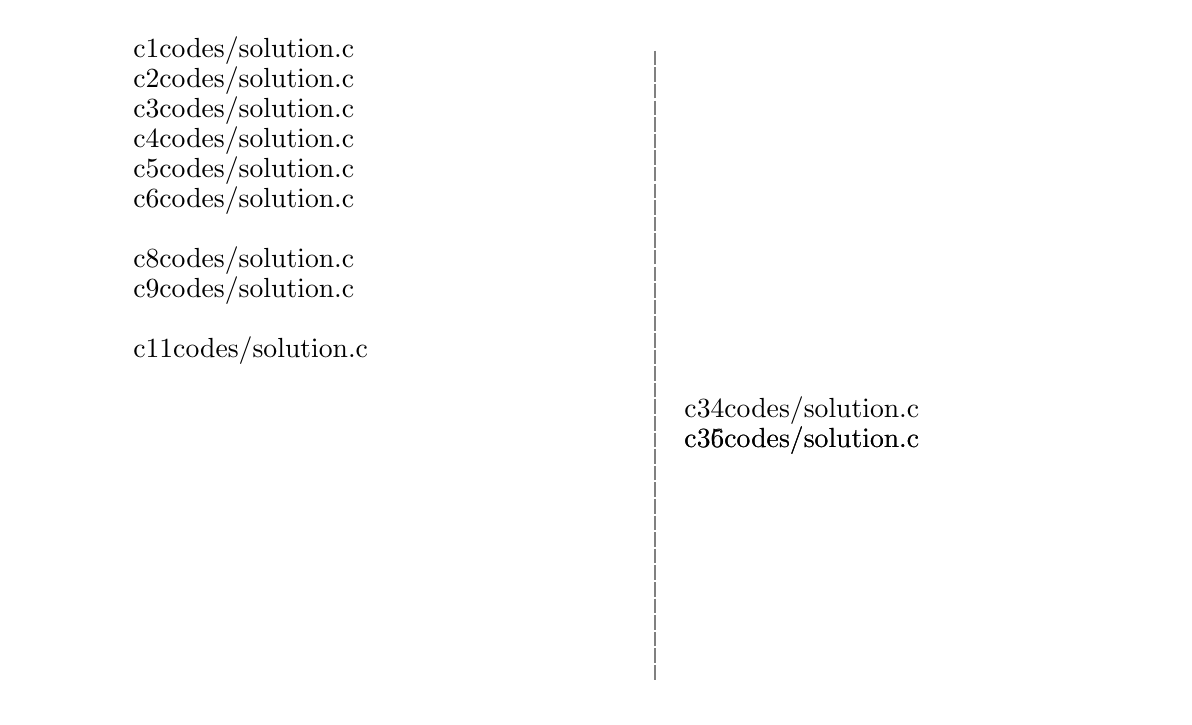
\begin{tikzpicture}
\node[draw,opacity=0] at (0, 0) {x};
\node[draw,opacity=0] at (14, 8) {x};

	\node[anchor=west] (line1) at (1.0, 8.0) { \inputline{c}{1}{codes/solution.c} };

	\node[anchor=west] (line2) at (1.0, 7.62) { \inputline{c}{2}{codes/solution.c} };

	\node[anchor=west] (line3) at (1.0, 7.24) { \inputline{c}{3}{codes/solution.c} };

	\node[anchor=west] (line4) at (1.0, 6.86) { \inputline{c}{4}{codes/solution.c} };

	\node[anchor=west] (line5) at (1.0, 6.48) { \inputline{c}{5}{codes/solution.c} };

	\node[anchor=west] (line6) at (1.0, 6.1) { \inputline{c}{6}{codes/solution.c} };


	\node[anchor=west] (line8) at (1.0, 5.33) { \inputline{c}{8}{codes/solution.c} };

	\node[anchor=west] (line9) at (1.0, 4.95) { \inputline{c}{9}{codes/solution.c} };


	\node[anchor=west] (line11) at (1.0, 4.19) { \inputline{c}{11}{codes/solution.c} };












	\draw[color=gray,dashed] (7.75, 8) -- (7.75, 0) -- cycle;











	\node[anchor=west] (line34) at (8.0, 3.43) { \inputline{c}{34}{codes/solution.c} };

	\node[anchor=west] (line35) at (8.0, 3.05) { \inputline{c}{35}{codes/solution.c} };

	\node[anchor=west] (line36) at (8.0, 3.05) { \inputline{c}{36}{codes/solution.c} };









\end{tikzpicture}
\end{frame}
\begin{frame}[plain,t]
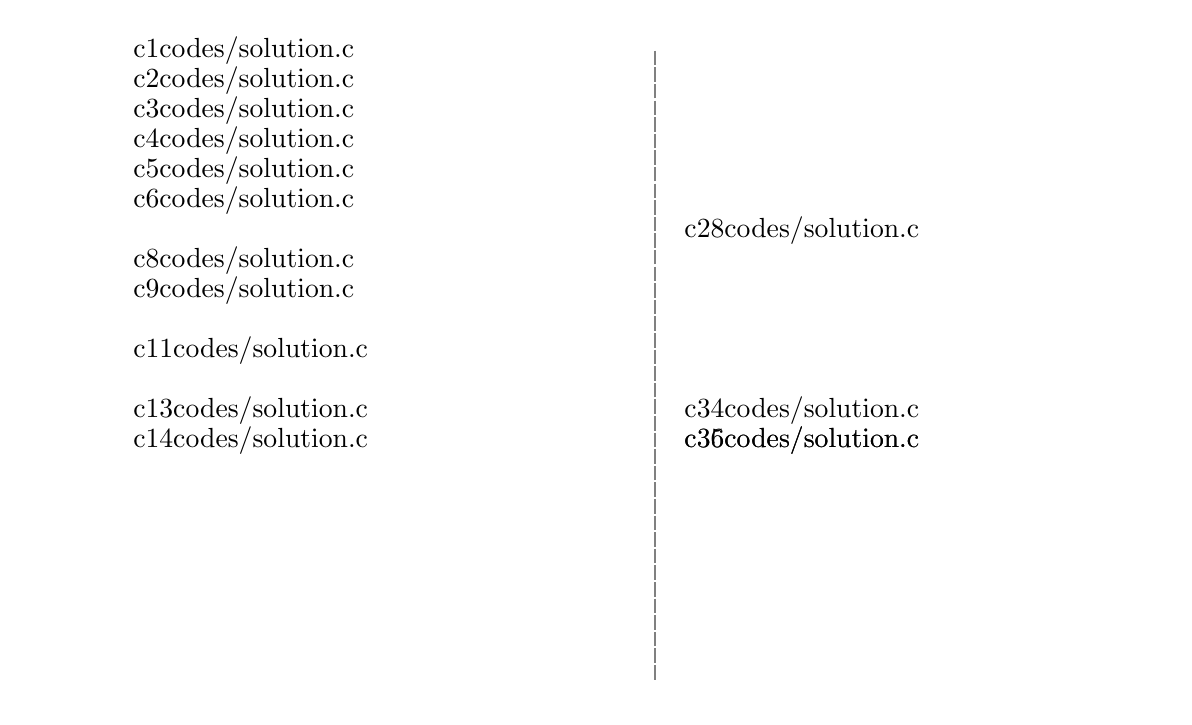
\begin{tikzpicture}
\node[draw,opacity=0] at (0, 0) {x};
\node[draw,opacity=0] at (14, 8) {x};

	\node[anchor=west] (line1) at (1.0, 8.0) { \inputline{c}{1}{codes/solution.c} };

	\node[anchor=west] (line2) at (1.0, 7.62) { \inputline{c}{2}{codes/solution.c} };

	\node[anchor=west] (line3) at (1.0, 7.24) { \inputline{c}{3}{codes/solution.c} };

	\node[anchor=west] (line4) at (1.0, 6.86) { \inputline{c}{4}{codes/solution.c} };

	\node[anchor=west] (line5) at (1.0, 6.48) { \inputline{c}{5}{codes/solution.c} };

	\node[anchor=west] (line6) at (1.0, 6.1) { \inputline{c}{6}{codes/solution.c} };


	\node[anchor=west] (line8) at (1.0, 5.33) { \inputline{c}{8}{codes/solution.c} };

	\node[anchor=west] (line9) at (1.0, 4.95) { \inputline{c}{9}{codes/solution.c} };


	\node[anchor=west] (line11) at (1.0, 4.19) { \inputline{c}{11}{codes/solution.c} };


	\node[anchor=west] (line13) at (1.0, 3.43) { \inputline{c}{13}{codes/solution.c} };

	\node[anchor=west] (line14) at (1.0, 3.05) { \inputline{c}{14}{codes/solution.c} };









	\draw[color=gray,dashed] (7.75, 8) -- (7.75, 0) -- cycle;





	\node[anchor=west] (line28) at (8.0, 5.71) { \inputline{c}{28}{codes/solution.c} };






	\node[anchor=west] (line34) at (8.0, 3.43) { \inputline{c}{34}{codes/solution.c} };

	\node[anchor=west] (line35) at (8.0, 3.05) { \inputline{c}{35}{codes/solution.c} };

	\node[anchor=west] (line36) at (8.0, 3.05) { \inputline{c}{36}{codes/solution.c} };











\end{tikzpicture}
\end{frame}
\begin{frame}[plain,t]
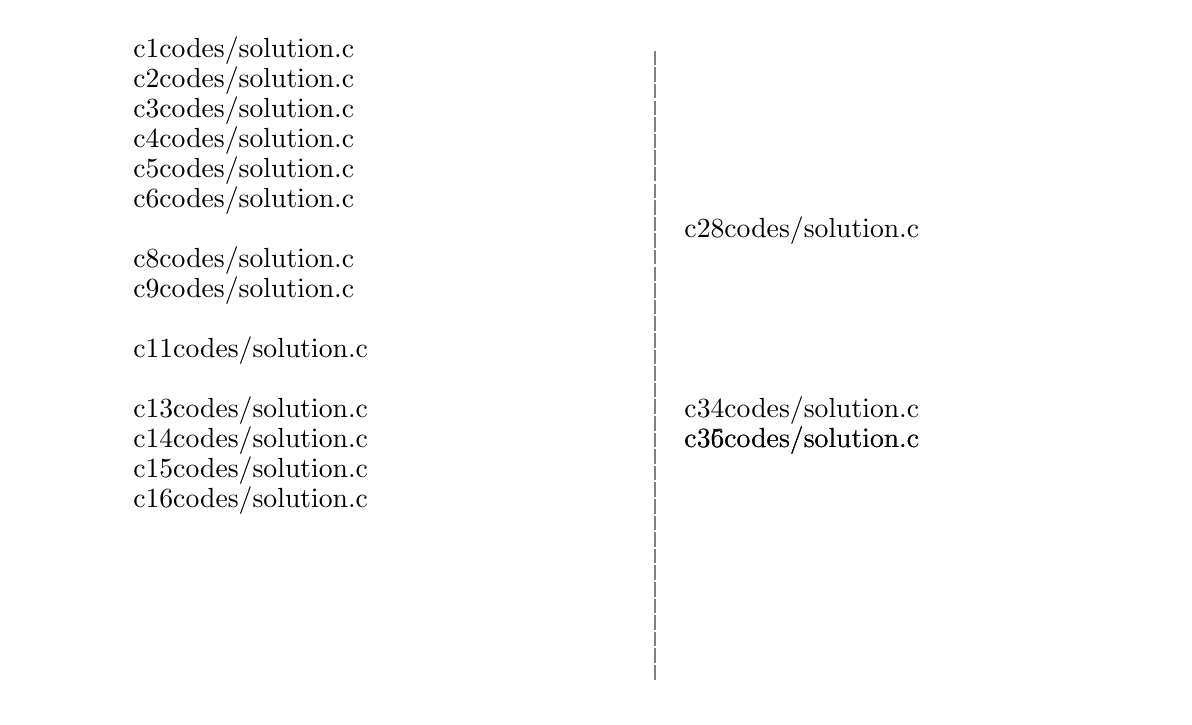
\begin{tikzpicture}
\node[draw,opacity=0] at (0, 0) {x};
\node[draw,opacity=0] at (14, 8) {x};

	\node[anchor=west] (line1) at (1.0, 8.0) { \inputline{c}{1}{codes/solution.c} };

	\node[anchor=west] (line2) at (1.0, 7.62) { \inputline{c}{2}{codes/solution.c} };

	\node[anchor=west] (line3) at (1.0, 7.24) { \inputline{c}{3}{codes/solution.c} };

	\node[anchor=west] (line4) at (1.0, 6.86) { \inputline{c}{4}{codes/solution.c} };

	\node[anchor=west] (line5) at (1.0, 6.48) { \inputline{c}{5}{codes/solution.c} };

	\node[anchor=west] (line6) at (1.0, 6.1) { \inputline{c}{6}{codes/solution.c} };


	\node[anchor=west] (line8) at (1.0, 5.33) { \inputline{c}{8}{codes/solution.c} };

	\node[anchor=west] (line9) at (1.0, 4.95) { \inputline{c}{9}{codes/solution.c} };


	\node[anchor=west] (line11) at (1.0, 4.19) { \inputline{c}{11}{codes/solution.c} };


	\node[anchor=west] (line13) at (1.0, 3.43) { \inputline{c}{13}{codes/solution.c} };

	\node[anchor=west] (line14) at (1.0, 3.05) { \inputline{c}{14}{codes/solution.c} };

	\node[anchor=west] (line15) at (1.0, 2.67) { \inputline{c}{15}{codes/solution.c} };

	\node[anchor=west] (line16) at (1.0, 2.29) { \inputline{c}{16}{codes/solution.c} };







	\draw[color=gray,dashed] (7.75, 8) -- (7.75, 0) -- cycle;





	\node[anchor=west] (line28) at (8.0, 5.71) { \inputline{c}{28}{codes/solution.c} };






	\node[anchor=west] (line34) at (8.0, 3.43) { \inputline{c}{34}{codes/solution.c} };

	\node[anchor=west] (line35) at (8.0, 3.05) { \inputline{c}{35}{codes/solution.c} };

	\node[anchor=west] (line36) at (8.0, 3.05) { \inputline{c}{36}{codes/solution.c} };













\end{tikzpicture}
\end{frame}
\begin{frame}[plain,t]
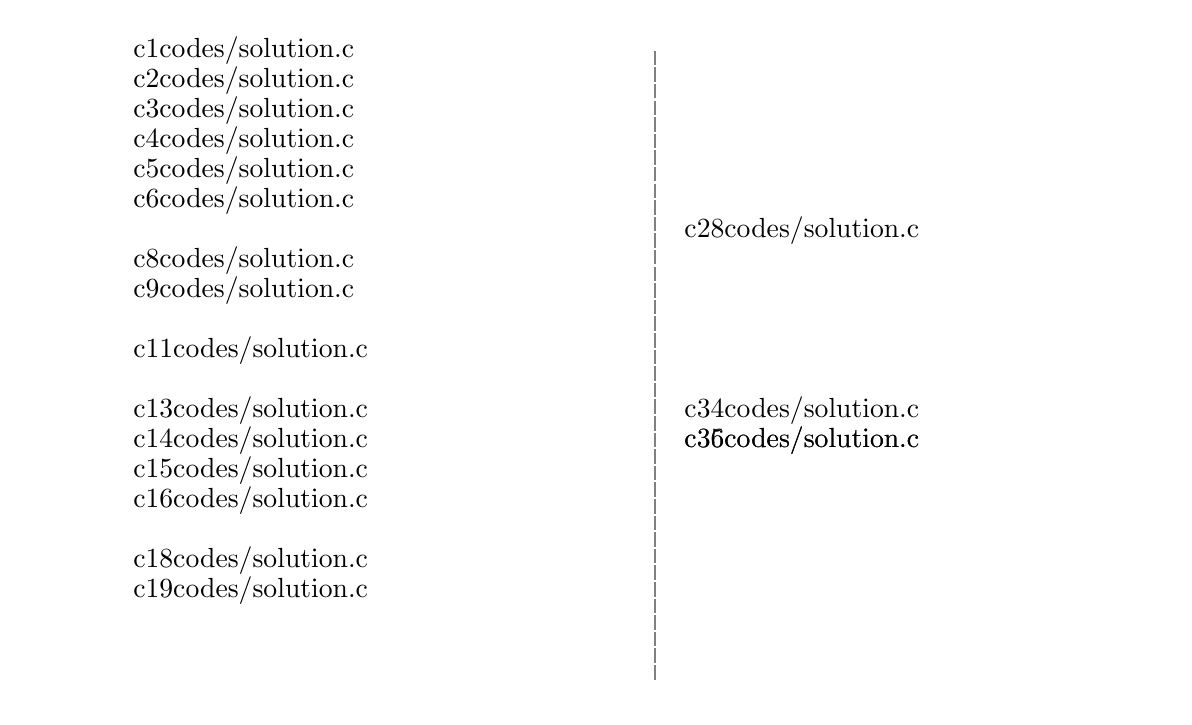
\begin{tikzpicture}
\node[draw,opacity=0] at (0, 0) {x};
\node[draw,opacity=0] at (14, 8) {x};

	\node[anchor=west] (line1) at (1.0, 8.0) { \inputline{c}{1}{codes/solution.c} };

	\node[anchor=west] (line2) at (1.0, 7.62) { \inputline{c}{2}{codes/solution.c} };

	\node[anchor=west] (line3) at (1.0, 7.24) { \inputline{c}{3}{codes/solution.c} };

	\node[anchor=west] (line4) at (1.0, 6.86) { \inputline{c}{4}{codes/solution.c} };

	\node[anchor=west] (line5) at (1.0, 6.48) { \inputline{c}{5}{codes/solution.c} };

	\node[anchor=west] (line6) at (1.0, 6.1) { \inputline{c}{6}{codes/solution.c} };


	\node[anchor=west] (line8) at (1.0, 5.33) { \inputline{c}{8}{codes/solution.c} };

	\node[anchor=west] (line9) at (1.0, 4.95) { \inputline{c}{9}{codes/solution.c} };


	\node[anchor=west] (line11) at (1.0, 4.19) { \inputline{c}{11}{codes/solution.c} };


	\node[anchor=west] (line13) at (1.0, 3.43) { \inputline{c}{13}{codes/solution.c} };

	\node[anchor=west] (line14) at (1.0, 3.05) { \inputline{c}{14}{codes/solution.c} };

	\node[anchor=west] (line15) at (1.0, 2.67) { \inputline{c}{15}{codes/solution.c} };

	\node[anchor=west] (line16) at (1.0, 2.29) { \inputline{c}{16}{codes/solution.c} };


	\node[anchor=west] (line18) at (1.0, 1.52) { \inputline{c}{18}{codes/solution.c} };

	\node[anchor=west] (line19) at (1.0, 1.14) { \inputline{c}{19}{codes/solution.c} };




	\draw[color=gray,dashed] (7.75, 8) -- (7.75, 0) -- cycle;





	\node[anchor=west] (line28) at (8.0, 5.71) { \inputline{c}{28}{codes/solution.c} };






	\node[anchor=west] (line34) at (8.0, 3.43) { \inputline{c}{34}{codes/solution.c} };

	\node[anchor=west] (line35) at (8.0, 3.05) { \inputline{c}{35}{codes/solution.c} };

	\node[anchor=west] (line36) at (8.0, 3.05) { \inputline{c}{36}{codes/solution.c} };















\end{tikzpicture}
\end{frame}
\begin{frame}[plain,t]
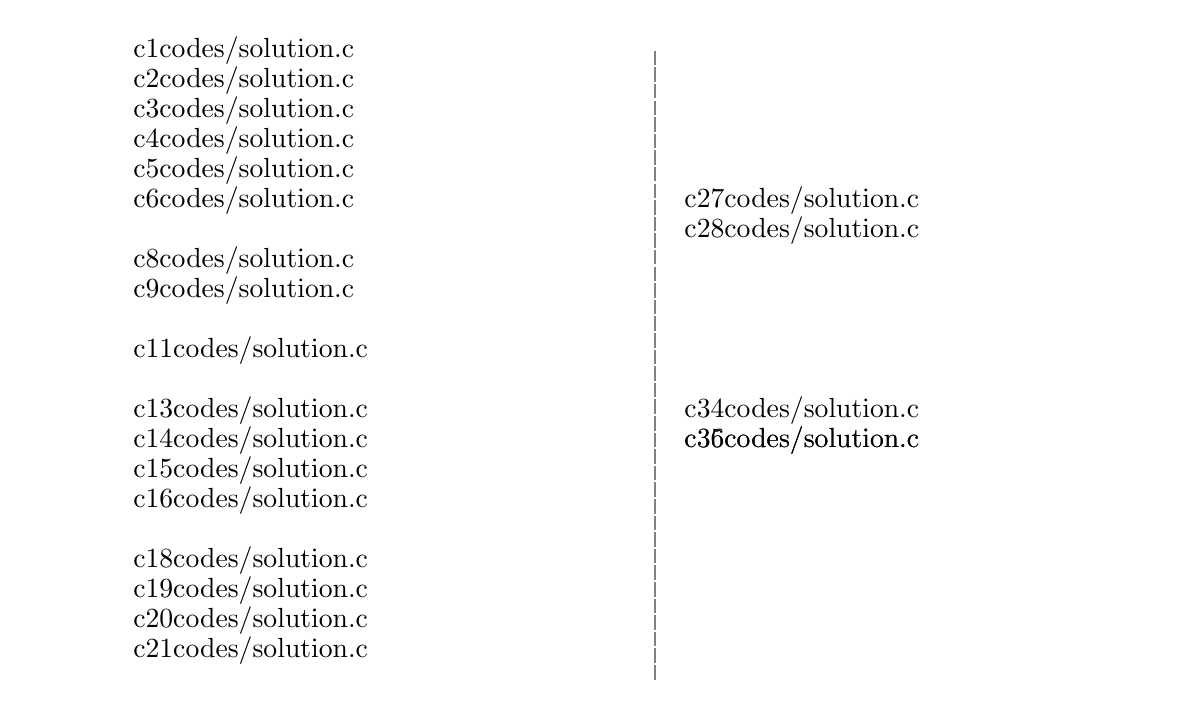
\begin{tikzpicture}
\node[draw,opacity=0] at (0, 0) {x};
\node[draw,opacity=0] at (14, 8) {x};

	\node[anchor=west] (line1) at (1.0, 8.0) { \inputline{c}{1}{codes/solution.c} };

	\node[anchor=west] (line2) at (1.0, 7.62) { \inputline{c}{2}{codes/solution.c} };

	\node[anchor=west] (line3) at (1.0, 7.24) { \inputline{c}{3}{codes/solution.c} };

	\node[anchor=west] (line4) at (1.0, 6.86) { \inputline{c}{4}{codes/solution.c} };

	\node[anchor=west] (line5) at (1.0, 6.48) { \inputline{c}{5}{codes/solution.c} };

	\node[anchor=west] (line6) at (1.0, 6.1) { \inputline{c}{6}{codes/solution.c} };


	\node[anchor=west] (line8) at (1.0, 5.33) { \inputline{c}{8}{codes/solution.c} };

	\node[anchor=west] (line9) at (1.0, 4.95) { \inputline{c}{9}{codes/solution.c} };


	\node[anchor=west] (line11) at (1.0, 4.19) { \inputline{c}{11}{codes/solution.c} };


	\node[anchor=west] (line13) at (1.0, 3.43) { \inputline{c}{13}{codes/solution.c} };

	\node[anchor=west] (line14) at (1.0, 3.05) { \inputline{c}{14}{codes/solution.c} };

	\node[anchor=west] (line15) at (1.0, 2.67) { \inputline{c}{15}{codes/solution.c} };

	\node[anchor=west] (line16) at (1.0, 2.29) { \inputline{c}{16}{codes/solution.c} };


	\node[anchor=west] (line18) at (1.0, 1.52) { \inputline{c}{18}{codes/solution.c} };

	\node[anchor=west] (line19) at (1.0, 1.14) { \inputline{c}{19}{codes/solution.c} };

	\node[anchor=west] (line20) at (1.0, 0.76) { \inputline{c}{20}{codes/solution.c} };

	\node[anchor=west] (line21) at (1.0, 0.38) { \inputline{c}{21}{codes/solution.c} };


	\draw[color=gray,dashed] (7.75, 8) -- (7.75, 0) -- cycle;




	\node[anchor=west] (line27) at (8.0, 6.1) { \inputline{c}{27}{codes/solution.c} };

	\node[anchor=west] (line28) at (8.0, 5.71) { \inputline{c}{28}{codes/solution.c} };






	\node[anchor=west] (line34) at (8.0, 3.43) { \inputline{c}{34}{codes/solution.c} };

	\node[anchor=west] (line35) at (8.0, 3.05) { \inputline{c}{35}{codes/solution.c} };

	\node[anchor=west] (line36) at (8.0, 3.05) { \inputline{c}{36}{codes/solution.c} };

















\end{tikzpicture}
\end{frame}
\begin{frame}[plain,t]
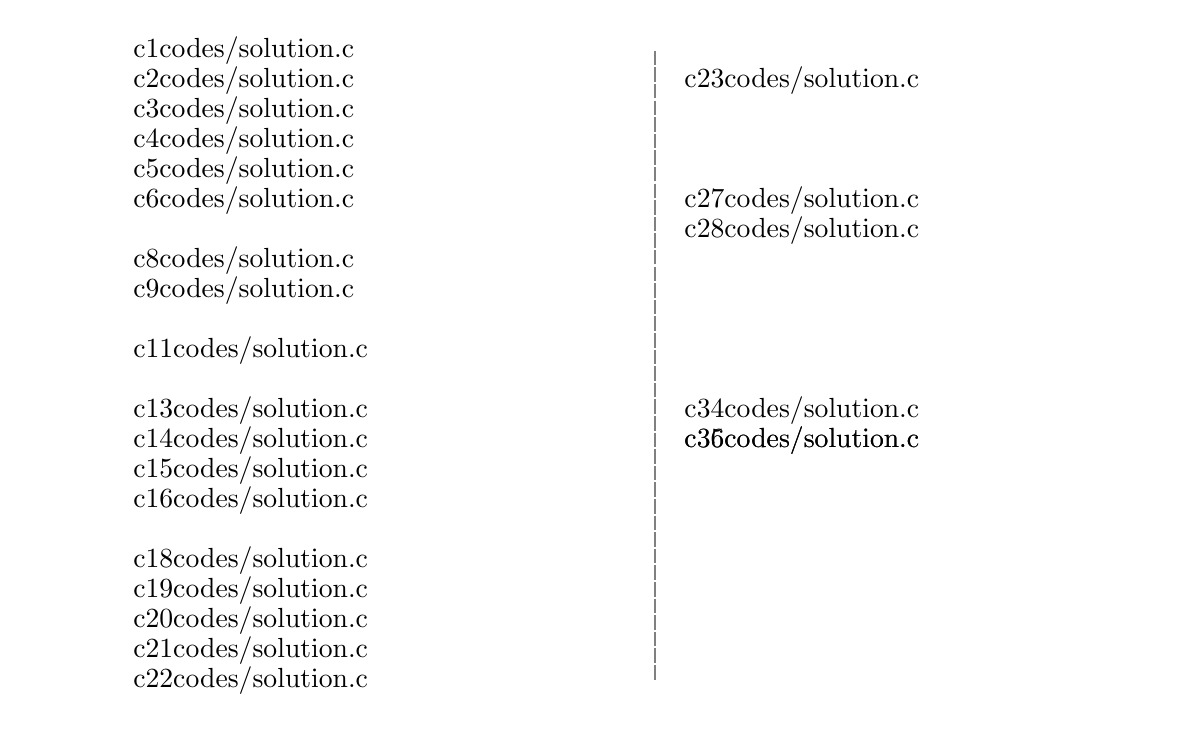
\begin{tikzpicture}
\node[draw,opacity=0] at (0, 0) {x};
\node[draw,opacity=0] at (14, 8) {x};

	\node[anchor=west] (line1) at (1.0, 8.0) { \inputline{c}{1}{codes/solution.c} };

	\node[anchor=west] (line2) at (1.0, 7.62) { \inputline{c}{2}{codes/solution.c} };

	\node[anchor=west] (line3) at (1.0, 7.24) { \inputline{c}{3}{codes/solution.c} };

	\node[anchor=west] (line4) at (1.0, 6.86) { \inputline{c}{4}{codes/solution.c} };

	\node[anchor=west] (line5) at (1.0, 6.48) { \inputline{c}{5}{codes/solution.c} };

	\node[anchor=west] (line6) at (1.0, 6.1) { \inputline{c}{6}{codes/solution.c} };


	\node[anchor=west] (line8) at (1.0, 5.33) { \inputline{c}{8}{codes/solution.c} };

	\node[anchor=west] (line9) at (1.0, 4.95) { \inputline{c}{9}{codes/solution.c} };


	\node[anchor=west] (line11) at (1.0, 4.19) { \inputline{c}{11}{codes/solution.c} };


	\node[anchor=west] (line13) at (1.0, 3.43) { \inputline{c}{13}{codes/solution.c} };

	\node[anchor=west] (line14) at (1.0, 3.05) { \inputline{c}{14}{codes/solution.c} };

	\node[anchor=west] (line15) at (1.0, 2.67) { \inputline{c}{15}{codes/solution.c} };

	\node[anchor=west] (line16) at (1.0, 2.29) { \inputline{c}{16}{codes/solution.c} };


	\node[anchor=west] (line18) at (1.0, 1.52) { \inputline{c}{18}{codes/solution.c} };

	\node[anchor=west] (line19) at (1.0, 1.14) { \inputline{c}{19}{codes/solution.c} };

	\node[anchor=west] (line20) at (1.0, 0.76) { \inputline{c}{20}{codes/solution.c} };

	\node[anchor=west] (line21) at (1.0, 0.38) { \inputline{c}{21}{codes/solution.c} };

	\node[anchor=west] (line22) at (1.0, -0.0) { \inputline{c}{22}{codes/solution.c} };

	\draw[color=gray,dashed] (7.75, 8) -- (7.75, 0) -- cycle;
	\node[anchor=west] (line23) at (8.0, 7.62) { \inputline{c}{23}{codes/solution.c} };




	\node[anchor=west] (line27) at (8.0, 6.1) { \inputline{c}{27}{codes/solution.c} };

	\node[anchor=west] (line28) at (8.0, 5.71) { \inputline{c}{28}{codes/solution.c} };






	\node[anchor=west] (line34) at (8.0, 3.43) { \inputline{c}{34}{codes/solution.c} };

	\node[anchor=west] (line35) at (8.0, 3.05) { \inputline{c}{35}{codes/solution.c} };

	\node[anchor=west] (line36) at (8.0, 3.05) { \inputline{c}{36}{codes/solution.c} };



















\end{tikzpicture}
\end{frame}
\begin{frame}[plain,t]
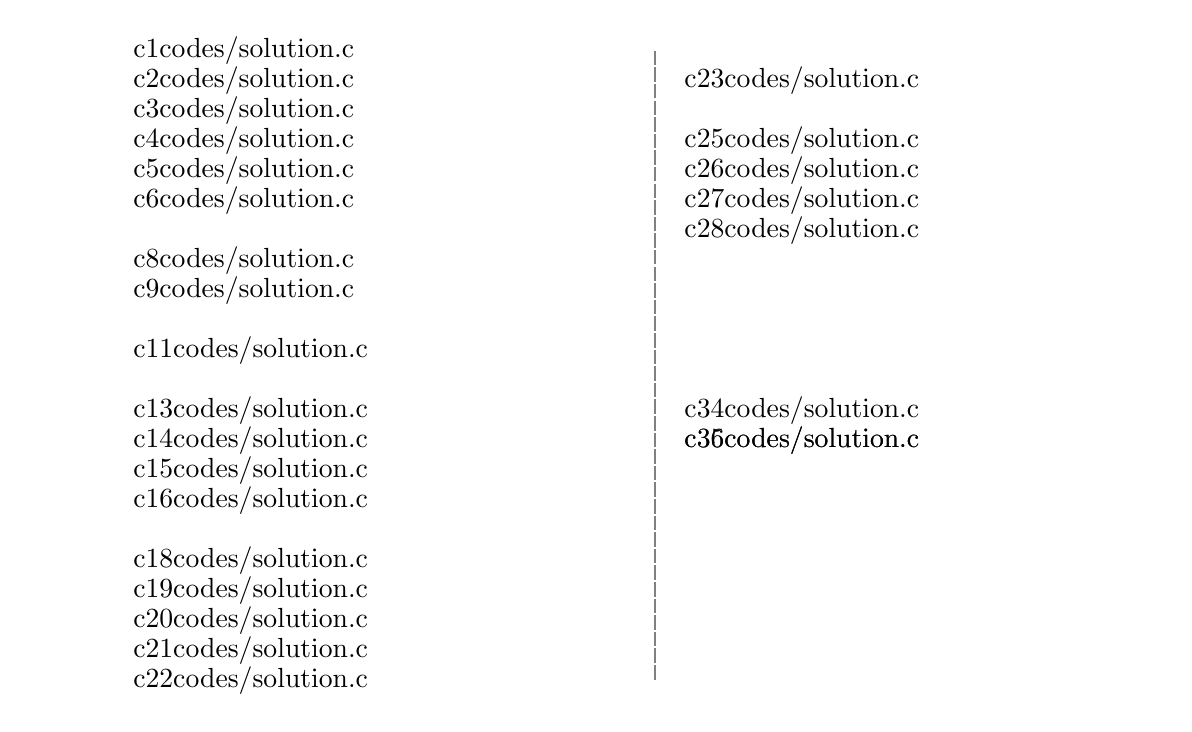
\begin{tikzpicture}
\node[draw,opacity=0] at (0, 0) {x};
\node[draw,opacity=0] at (14, 8) {x};

	\node[anchor=west] (line1) at (1.0, 8.0) { \inputline{c}{1}{codes/solution.c} };

	\node[anchor=west] (line2) at (1.0, 7.62) { \inputline{c}{2}{codes/solution.c} };

	\node[anchor=west] (line3) at (1.0, 7.24) { \inputline{c}{3}{codes/solution.c} };

	\node[anchor=west] (line4) at (1.0, 6.86) { \inputline{c}{4}{codes/solution.c} };

	\node[anchor=west] (line5) at (1.0, 6.48) { \inputline{c}{5}{codes/solution.c} };

	\node[anchor=west] (line6) at (1.0, 6.1) { \inputline{c}{6}{codes/solution.c} };


	\node[anchor=west] (line8) at (1.0, 5.33) { \inputline{c}{8}{codes/solution.c} };

	\node[anchor=west] (line9) at (1.0, 4.95) { \inputline{c}{9}{codes/solution.c} };


	\node[anchor=west] (line11) at (1.0, 4.19) { \inputline{c}{11}{codes/solution.c} };


	\node[anchor=west] (line13) at (1.0, 3.43) { \inputline{c}{13}{codes/solution.c} };

	\node[anchor=west] (line14) at (1.0, 3.05) { \inputline{c}{14}{codes/solution.c} };

	\node[anchor=west] (line15) at (1.0, 2.67) { \inputline{c}{15}{codes/solution.c} };

	\node[anchor=west] (line16) at (1.0, 2.29) { \inputline{c}{16}{codes/solution.c} };


	\node[anchor=west] (line18) at (1.0, 1.52) { \inputline{c}{18}{codes/solution.c} };

	\node[anchor=west] (line19) at (1.0, 1.14) { \inputline{c}{19}{codes/solution.c} };

	\node[anchor=west] (line20) at (1.0, 0.76) { \inputline{c}{20}{codes/solution.c} };

	\node[anchor=west] (line21) at (1.0, 0.38) { \inputline{c}{21}{codes/solution.c} };

	\node[anchor=west] (line22) at (1.0, -0.0) { \inputline{c}{22}{codes/solution.c} };

	\draw[color=gray,dashed] (7.75, 8) -- (7.75, 0) -- cycle;
	\node[anchor=west] (line23) at (8.0, 7.62) { \inputline{c}{23}{codes/solution.c} };


	\node[anchor=west] (line25) at (8.0, 6.86) { \inputline{c}{25}{codes/solution.c} };

	\node[anchor=west] (line26) at (8.0, 6.48) { \inputline{c}{26}{codes/solution.c} };

	\node[anchor=west] (line27) at (8.0, 6.1) { \inputline{c}{27}{codes/solution.c} };

	\node[anchor=west] (line28) at (8.0, 5.71) { \inputline{c}{28}{codes/solution.c} };






	\node[anchor=west] (line34) at (8.0, 3.43) { \inputline{c}{34}{codes/solution.c} };

	\node[anchor=west] (line35) at (8.0, 3.05) { \inputline{c}{35}{codes/solution.c} };

	\node[anchor=west] (line36) at (8.0, 3.05) { \inputline{c}{36}{codes/solution.c} };





















\end{tikzpicture}
\end{frame}
\begin{frame}[plain,t]
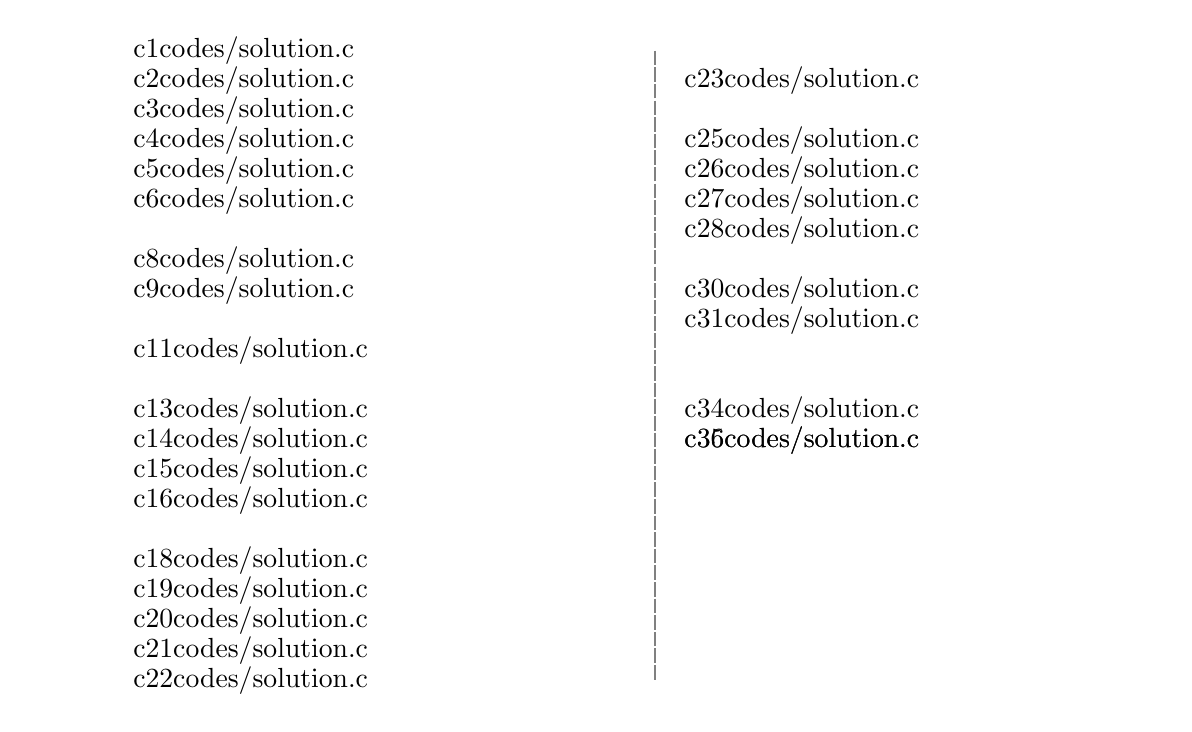
\begin{tikzpicture}
\node[draw,opacity=0] at (0, 0) {x};
\node[draw,opacity=0] at (14, 8) {x};

	\node[anchor=west] (line1) at (1.0, 8.0) { \inputline{c}{1}{codes/solution.c} };

	\node[anchor=west] (line2) at (1.0, 7.62) { \inputline{c}{2}{codes/solution.c} };

	\node[anchor=west] (line3) at (1.0, 7.24) { \inputline{c}{3}{codes/solution.c} };

	\node[anchor=west] (line4) at (1.0, 6.86) { \inputline{c}{4}{codes/solution.c} };

	\node[anchor=west] (line5) at (1.0, 6.48) { \inputline{c}{5}{codes/solution.c} };

	\node[anchor=west] (line6) at (1.0, 6.1) { \inputline{c}{6}{codes/solution.c} };


	\node[anchor=west] (line8) at (1.0, 5.33) { \inputline{c}{8}{codes/solution.c} };

	\node[anchor=west] (line9) at (1.0, 4.95) { \inputline{c}{9}{codes/solution.c} };


	\node[anchor=west] (line11) at (1.0, 4.19) { \inputline{c}{11}{codes/solution.c} };


	\node[anchor=west] (line13) at (1.0, 3.43) { \inputline{c}{13}{codes/solution.c} };

	\node[anchor=west] (line14) at (1.0, 3.05) { \inputline{c}{14}{codes/solution.c} };

	\node[anchor=west] (line15) at (1.0, 2.67) { \inputline{c}{15}{codes/solution.c} };

	\node[anchor=west] (line16) at (1.0, 2.29) { \inputline{c}{16}{codes/solution.c} };


	\node[anchor=west] (line18) at (1.0, 1.52) { \inputline{c}{18}{codes/solution.c} };

	\node[anchor=west] (line19) at (1.0, 1.14) { \inputline{c}{19}{codes/solution.c} };

	\node[anchor=west] (line20) at (1.0, 0.76) { \inputline{c}{20}{codes/solution.c} };

	\node[anchor=west] (line21) at (1.0, 0.38) { \inputline{c}{21}{codes/solution.c} };

	\node[anchor=west] (line22) at (1.0, -0.0) { \inputline{c}{22}{codes/solution.c} };

	\draw[color=gray,dashed] (7.75, 8) -- (7.75, 0) -- cycle;
	\node[anchor=west] (line23) at (8.0, 7.62) { \inputline{c}{23}{codes/solution.c} };


	\node[anchor=west] (line25) at (8.0, 6.86) { \inputline{c}{25}{codes/solution.c} };

	\node[anchor=west] (line26) at (8.0, 6.48) { \inputline{c}{26}{codes/solution.c} };

	\node[anchor=west] (line27) at (8.0, 6.1) { \inputline{c}{27}{codes/solution.c} };

	\node[anchor=west] (line28) at (8.0, 5.71) { \inputline{c}{28}{codes/solution.c} };


	\node[anchor=west] (line30) at (8.0, 4.95) { \inputline{c}{30}{codes/solution.c} };

	\node[anchor=west] (line31) at (8.0, 4.57) { \inputline{c}{31}{codes/solution.c} };



	\node[anchor=west] (line34) at (8.0, 3.43) { \inputline{c}{34}{codes/solution.c} };

	\node[anchor=west] (line35) at (8.0, 3.05) { \inputline{c}{35}{codes/solution.c} };

	\node[anchor=west] (line36) at (8.0, 3.05) { \inputline{c}{36}{codes/solution.c} };























\end{tikzpicture}
\end{frame}
\begin{frame}[plain,t]
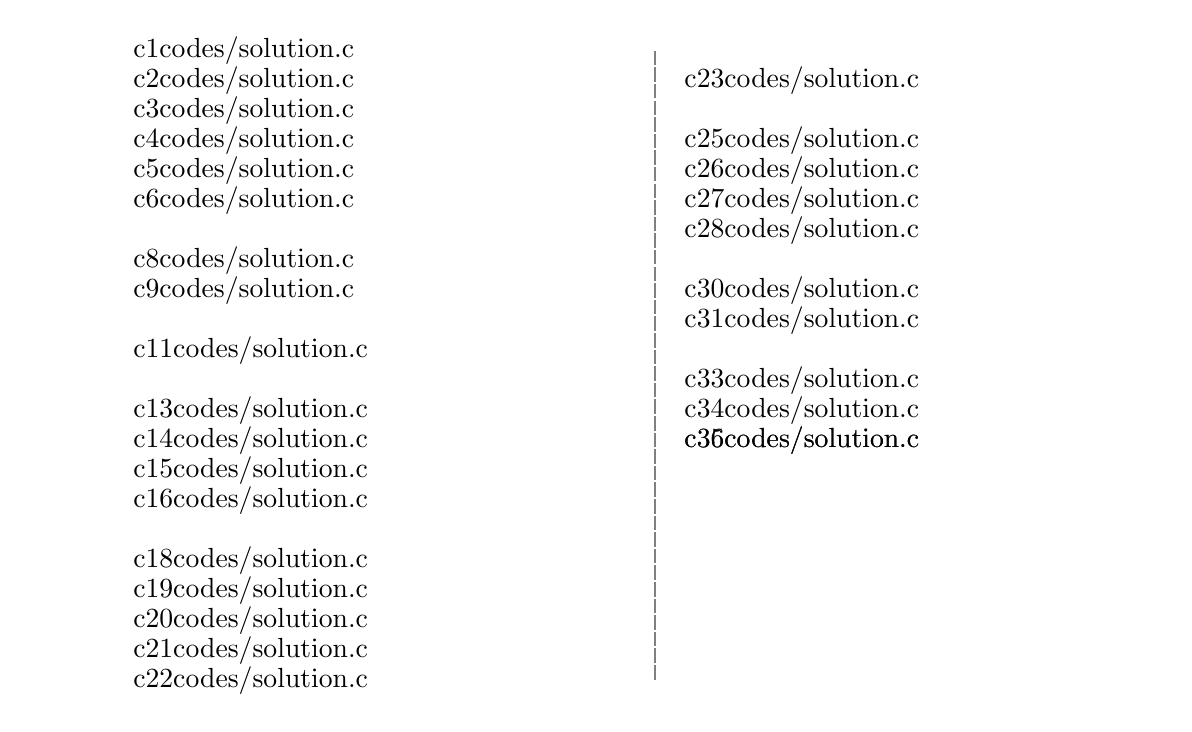
\begin{tikzpicture}
\node[draw,opacity=0] at (0, 0) {x};
\node[draw,opacity=0] at (14, 8) {x};

	\node[anchor=west] (line1) at (1.0, 8.0) { \inputline{c}{1}{codes/solution.c} };

	\node[anchor=west] (line2) at (1.0, 7.62) { \inputline{c}{2}{codes/solution.c} };

	\node[anchor=west] (line3) at (1.0, 7.24) { \inputline{c}{3}{codes/solution.c} };

	\node[anchor=west] (line4) at (1.0, 6.86) { \inputline{c}{4}{codes/solution.c} };

	\node[anchor=west] (line5) at (1.0, 6.48) { \inputline{c}{5}{codes/solution.c} };

	\node[anchor=west] (line6) at (1.0, 6.1) { \inputline{c}{6}{codes/solution.c} };


	\node[anchor=west] (line8) at (1.0, 5.33) { \inputline{c}{8}{codes/solution.c} };

	\node[anchor=west] (line9) at (1.0, 4.95) { \inputline{c}{9}{codes/solution.c} };


	\node[anchor=west] (line11) at (1.0, 4.19) { \inputline{c}{11}{codes/solution.c} };


	\node[anchor=west] (line13) at (1.0, 3.43) { \inputline{c}{13}{codes/solution.c} };

	\node[anchor=west] (line14) at (1.0, 3.05) { \inputline{c}{14}{codes/solution.c} };

	\node[anchor=west] (line15) at (1.0, 2.67) { \inputline{c}{15}{codes/solution.c} };

	\node[anchor=west] (line16) at (1.0, 2.29) { \inputline{c}{16}{codes/solution.c} };


	\node[anchor=west] (line18) at (1.0, 1.52) { \inputline{c}{18}{codes/solution.c} };

	\node[anchor=west] (line19) at (1.0, 1.14) { \inputline{c}{19}{codes/solution.c} };

	\node[anchor=west] (line20) at (1.0, 0.76) { \inputline{c}{20}{codes/solution.c} };

	\node[anchor=west] (line21) at (1.0, 0.38) { \inputline{c}{21}{codes/solution.c} };

	\node[anchor=west] (line22) at (1.0, -0.0) { \inputline{c}{22}{codes/solution.c} };

	\draw[color=gray,dashed] (7.75, 8) -- (7.75, 0) -- cycle;
	\node[anchor=west] (line23) at (8.0, 7.62) { \inputline{c}{23}{codes/solution.c} };


	\node[anchor=west] (line25) at (8.0, 6.86) { \inputline{c}{25}{codes/solution.c} };

	\node[anchor=west] (line26) at (8.0, 6.48) { \inputline{c}{26}{codes/solution.c} };

	\node[anchor=west] (line27) at (8.0, 6.1) { \inputline{c}{27}{codes/solution.c} };

	\node[anchor=west] (line28) at (8.0, 5.71) { \inputline{c}{28}{codes/solution.c} };


	\node[anchor=west] (line30) at (8.0, 4.95) { \inputline{c}{30}{codes/solution.c} };

	\node[anchor=west] (line31) at (8.0, 4.57) { \inputline{c}{31}{codes/solution.c} };


	\node[anchor=west] (line33) at (8.0, 3.81) { \inputline{c}{33}{codes/solution.c} };

	\node[anchor=west] (line34) at (8.0, 3.43) { \inputline{c}{34}{codes/solution.c} };

	\node[anchor=west] (line35) at (8.0, 3.05) { \inputline{c}{35}{codes/solution.c} };

	\node[anchor=west] (line36) at (8.0, 3.05) { \inputline{c}{36}{codes/solution.c} };

























\end{tikzpicture}
\end{frame}
\begin{frame}[plain,t]
\begin{tikzpicture}
\node[draw,opacity=0] at (0, 0) {x};
\node[draw,opacity=0] at (14, 8) {x};

	\node[anchor=west] (title) at (0.0, 7.0) { \Large \bbbold{Bônus} };

\end{tikzpicture}
\end{frame}
\begin{frame}[plain,t]
\begin{tikzpicture}
\node[draw,opacity=0] at (0, 0) {x};
\node[draw,opacity=0] at (14, 8) {x};

	\node[anchor=west] (title) at (0.0, 7.0) { \Large \bbbold{Bônus} };


	\node[anchor=west] (a) at (1.0, 6.0) { $\star$ \bbtext{Há uma solução alternativa para este problema} };

\end{tikzpicture}
\end{frame}
\begin{frame}[plain,t]
\begin{tikzpicture}
\node[draw,opacity=0] at (0, 0) {x};
\node[draw,opacity=0] at (14, 8) {x};

	\node[anchor=west] (title) at (0.0, 7.0) { \Large \bbbold{Bônus} };


	\node[anchor=west] (a) at (1.0, 6.0) { $\star$ \bbtext{Há uma solução alternativa para este problema} };


	\node[anchor=west] (b) at (1.0, 5.0) { $\star$ \bbtext{Ela é baseada em uma técnica denominada \bbbold{dois ponteiros}} };

\end{tikzpicture}
\end{frame}
\begin{frame}[plain,t]
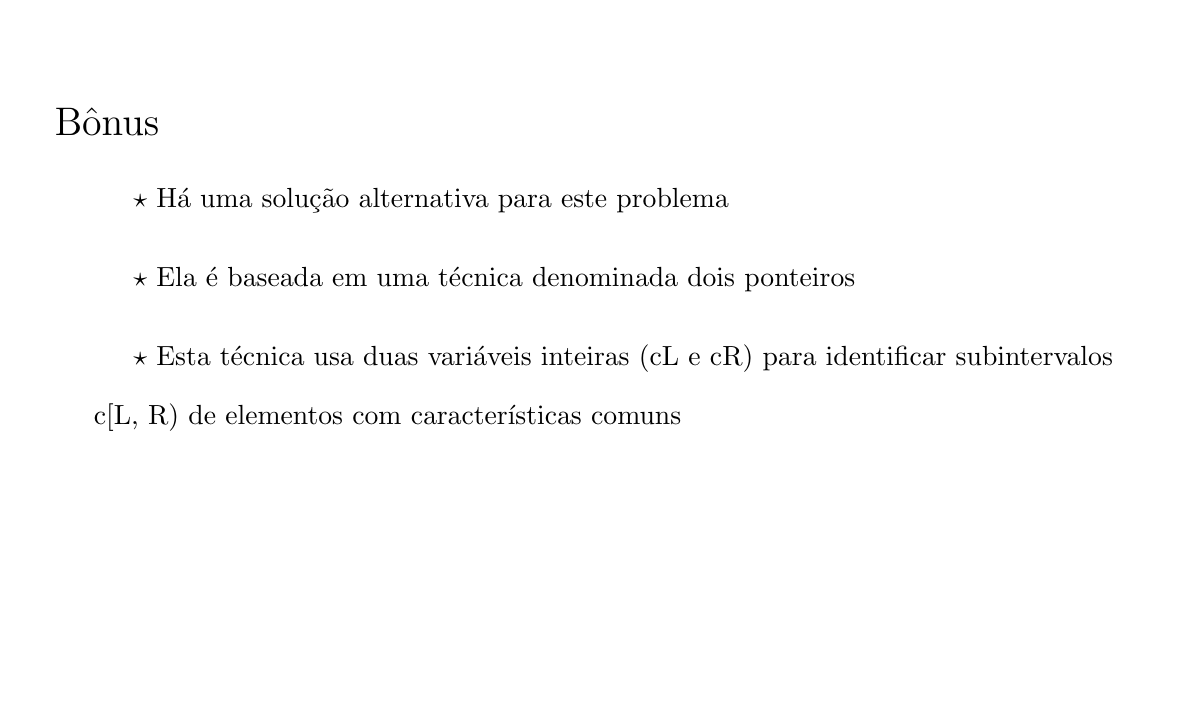
\begin{tikzpicture}
\node[draw,opacity=0] at (0, 0) {x};
\node[draw,opacity=0] at (14, 8) {x};

	\node[anchor=west] (title) at (0.0, 7.0) { \Large \bbbold{Bônus} };


	\node[anchor=west] (a) at (1.0, 6.0) { $\star$ \bbtext{Há uma solução alternativa para este problema} };


	\node[anchor=west] (b) at (1.0, 5.0) { $\star$ \bbtext{Ela é baseada em uma técnica denominada \bbbold{dois ponteiros}} };


	\node[anchor=west] (c) at (1.0, 4.0) { $\star$ \bbtext{Esta técnica usa duas variáveis inteiras (\code{c}{L} e \code{c}{R}) para identificar subintervalos} };

	\node[anchor=west] (c1) at (0.5, 3.25) { \bbtext{\code{c}{[L, R)} de elementos com características comuns} };

\end{tikzpicture}
\end{frame}
\begin{frame}[plain,t]
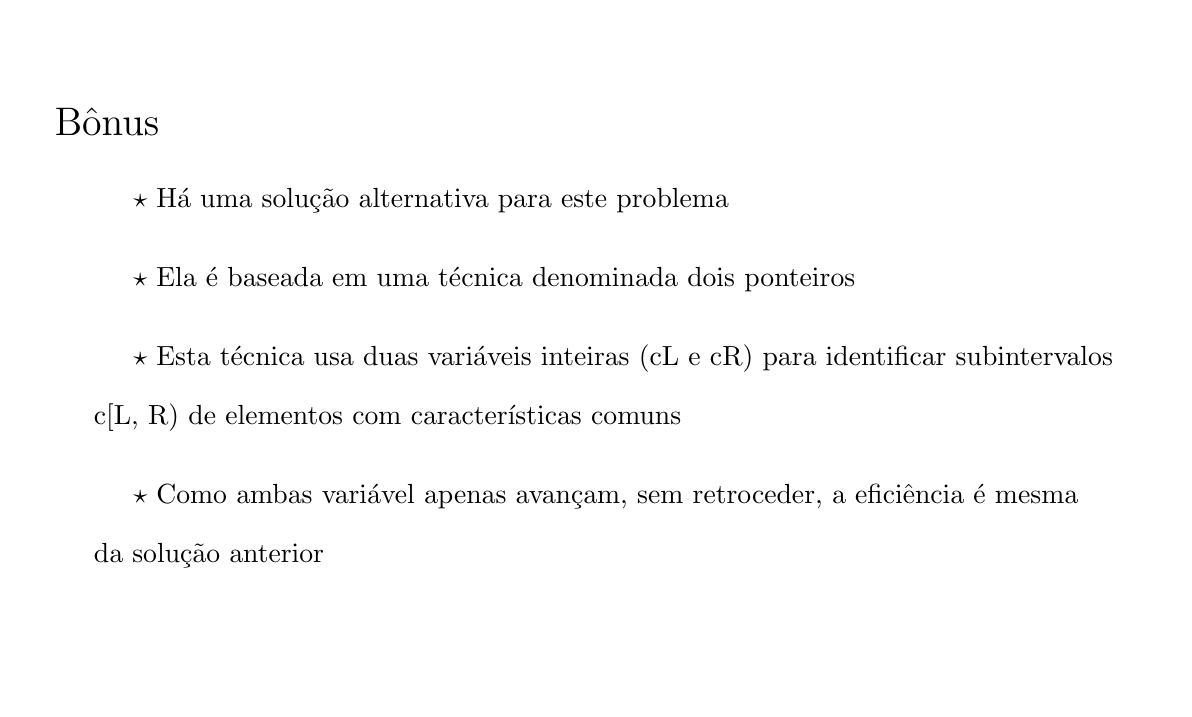
\begin{tikzpicture}
\node[draw,opacity=0] at (0, 0) {x};
\node[draw,opacity=0] at (14, 8) {x};

	\node[anchor=west] (title) at (0.0, 7.0) { \Large \bbbold{Bônus} };


	\node[anchor=west] (a) at (1.0, 6.0) { $\star$ \bbtext{Há uma solução alternativa para este problema} };


	\node[anchor=west] (b) at (1.0, 5.0) { $\star$ \bbtext{Ela é baseada em uma técnica denominada \bbbold{dois ponteiros}} };


	\node[anchor=west] (c) at (1.0, 4.0) { $\star$ \bbtext{Esta técnica usa duas variáveis inteiras (\code{c}{L} e \code{c}{R}) para identificar subintervalos} };

	\node[anchor=west] (c1) at (0.5, 3.25) { \bbtext{\code{c}{[L, R)} de elementos com características comuns} };


	\node[anchor=west] (d) at (1.0, 2.25) { $\star$ \bbtext{Como ambas variável apenas avançam, sem retroceder, a eficiência é mesma} };

	\node[anchor=west] (d1) at (0.5, 1.5) { \bbtext{da solução anterior} };

\end{tikzpicture}
\end{frame}
\begin{frame}[plain,t]
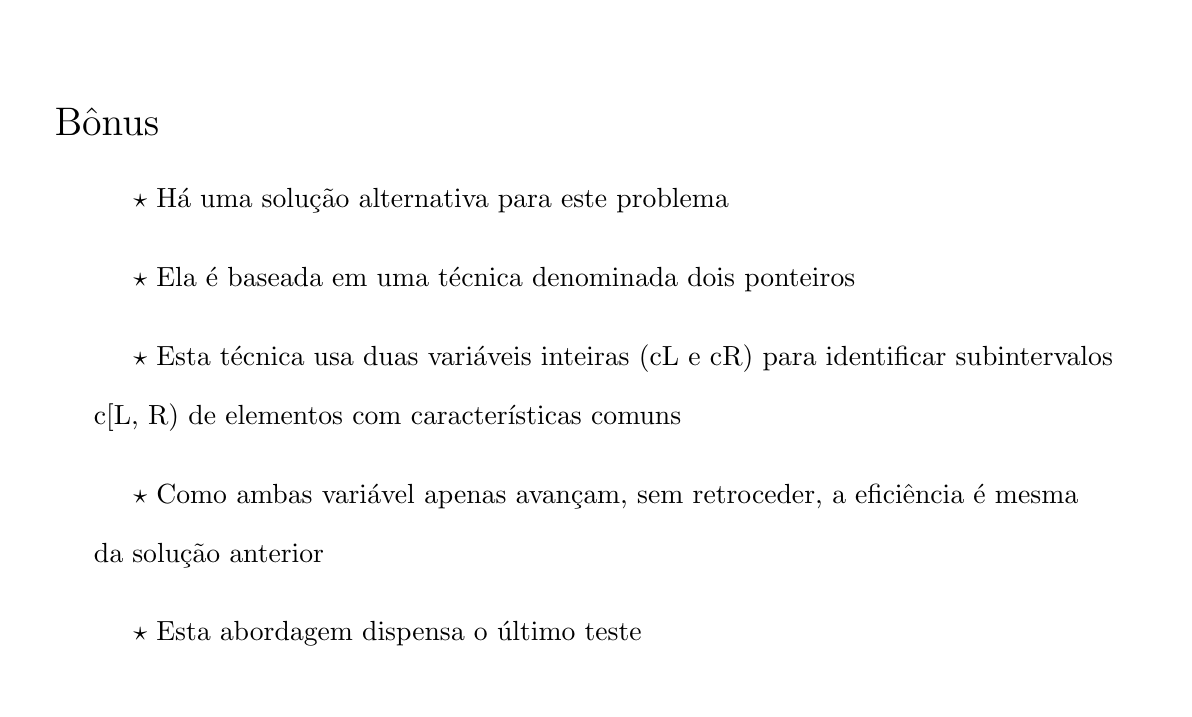
\begin{tikzpicture}
\node[draw,opacity=0] at (0, 0) {x};
\node[draw,opacity=0] at (14, 8) {x};

	\node[anchor=west] (title) at (0.0, 7.0) { \Large \bbbold{Bônus} };


	\node[anchor=west] (a) at (1.0, 6.0) { $\star$ \bbtext{Há uma solução alternativa para este problema} };


	\node[anchor=west] (b) at (1.0, 5.0) { $\star$ \bbtext{Ela é baseada em uma técnica denominada \bbbold{dois ponteiros}} };


	\node[anchor=west] (c) at (1.0, 4.0) { $\star$ \bbtext{Esta técnica usa duas variáveis inteiras (\code{c}{L} e \code{c}{R}) para identificar subintervalos} };

	\node[anchor=west] (c1) at (0.5, 3.25) { \bbtext{\code{c}{[L, R)} de elementos com características comuns} };


	\node[anchor=west] (d) at (1.0, 2.25) { $\star$ \bbtext{Como ambas variável apenas avançam, sem retroceder, a eficiência é mesma} };

	\node[anchor=west] (d1) at (0.5, 1.5) { \bbtext{da solução anterior} };


	\node[anchor=west] (e) at (1.0, 0.5) { $\star$ \bbtext{Esta abordagem dispensa o último teste} };

\end{tikzpicture}
\end{frame}
\begin{frame}[plain,t]
\begin{tikzpicture}
\node[draw,opacity=0] at (0, 0) {x};
\node[draw,opacity=0] at (14, 8) {x};

	\node[anchor=west] (line1) at (1.0, 8.0) { \inputline{c}{1}{codes/solution2.c} };

	\node[anchor=west] (line2) at (1.0, 7.62) { \inputline{c}{2}{codes/solution2.c} };

	\node[anchor=west] (line3) at (1.0, 7.24) { \inputline{c}{3}{codes/solution2.c} };

	\node[anchor=west] (line4) at (1.0, 6.86) { \inputline{c}{4}{codes/solution2.c} };

	\node[anchor=west] (line5) at (1.0, 6.48) { \inputline{c}{5}{codes/solution2.c} };

	\node[anchor=west] (line6) at (1.0, 6.1) { \inputline{c}{6}{codes/solution2.c} };

















	\draw[color=gray,dashed] (7.5, 8) -- (7.5, 0) -- cycle;







	\node[anchor=west] (line30) at (8.0, 4.95) { \inputline{c}{30}{codes/solution2.c} };

	\node[anchor=west] (line31) at (8.0, 4.57) { \inputline{c}{31}{codes/solution2.c} };


\end{tikzpicture}
\end{frame}
\begin{frame}[plain,t]
\begin{tikzpicture}
\node[draw,opacity=0] at (0, 0) {x};
\node[draw,opacity=0] at (14, 8) {x};

	\node[anchor=west] (line1) at (1.0, 8.0) { \inputline{c}{1}{codes/solution2.c} };

	\node[anchor=west] (line2) at (1.0, 7.62) { \inputline{c}{2}{codes/solution2.c} };

	\node[anchor=west] (line3) at (1.0, 7.24) { \inputline{c}{3}{codes/solution2.c} };

	\node[anchor=west] (line4) at (1.0, 6.86) { \inputline{c}{4}{codes/solution2.c} };

	\node[anchor=west] (line5) at (1.0, 6.48) { \inputline{c}{5}{codes/solution2.c} };

	\node[anchor=west] (line6) at (1.0, 6.1) { \inputline{c}{6}{codes/solution2.c} };


	\node[anchor=west] (line8) at (1.0, 5.33) { \inputline{c}{8}{codes/solution2.c} };















	\draw[color=gray,dashed] (7.5, 8) -- (7.5, 0) -- cycle;







	\node[anchor=west] (line30) at (8.0, 4.95) { \inputline{c}{30}{codes/solution2.c} };

	\node[anchor=west] (line31) at (8.0, 4.57) { \inputline{c}{31}{codes/solution2.c} };




\end{tikzpicture}
\end{frame}
\begin{frame}[plain,t]
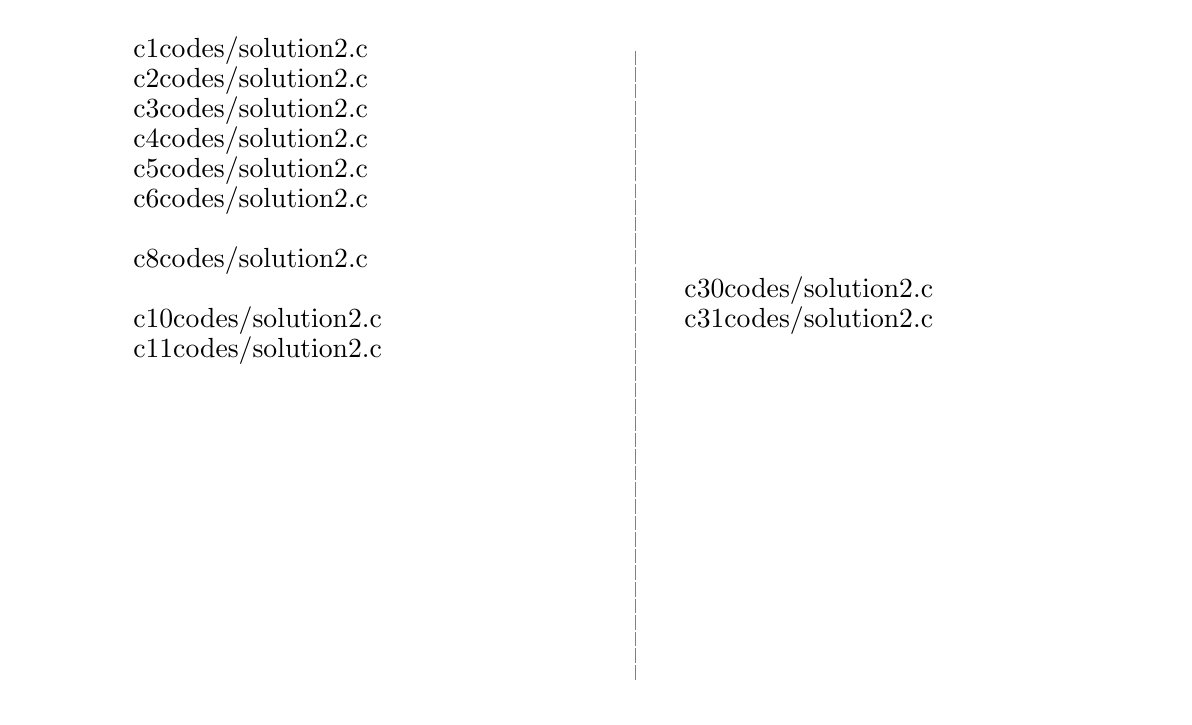
\begin{tikzpicture}
\node[draw,opacity=0] at (0, 0) {x};
\node[draw,opacity=0] at (14, 8) {x};

	\node[anchor=west] (line1) at (1.0, 8.0) { \inputline{c}{1}{codes/solution2.c} };

	\node[anchor=west] (line2) at (1.0, 7.62) { \inputline{c}{2}{codes/solution2.c} };

	\node[anchor=west] (line3) at (1.0, 7.24) { \inputline{c}{3}{codes/solution2.c} };

	\node[anchor=west] (line4) at (1.0, 6.86) { \inputline{c}{4}{codes/solution2.c} };

	\node[anchor=west] (line5) at (1.0, 6.48) { \inputline{c}{5}{codes/solution2.c} };

	\node[anchor=west] (line6) at (1.0, 6.1) { \inputline{c}{6}{codes/solution2.c} };


	\node[anchor=west] (line8) at (1.0, 5.33) { \inputline{c}{8}{codes/solution2.c} };


	\node[anchor=west] (line10) at (1.0, 4.57) { \inputline{c}{10}{codes/solution2.c} };

	\node[anchor=west] (line11) at (1.0, 4.19) { \inputline{c}{11}{codes/solution2.c} };












	\draw[color=gray,dashed] (7.5, 8) -- (7.5, 0) -- cycle;







	\node[anchor=west] (line30) at (8.0, 4.95) { \inputline{c}{30}{codes/solution2.c} };

	\node[anchor=west] (line31) at (8.0, 4.57) { \inputline{c}{31}{codes/solution2.c} };






\end{tikzpicture}
\end{frame}
\begin{frame}[plain,t]
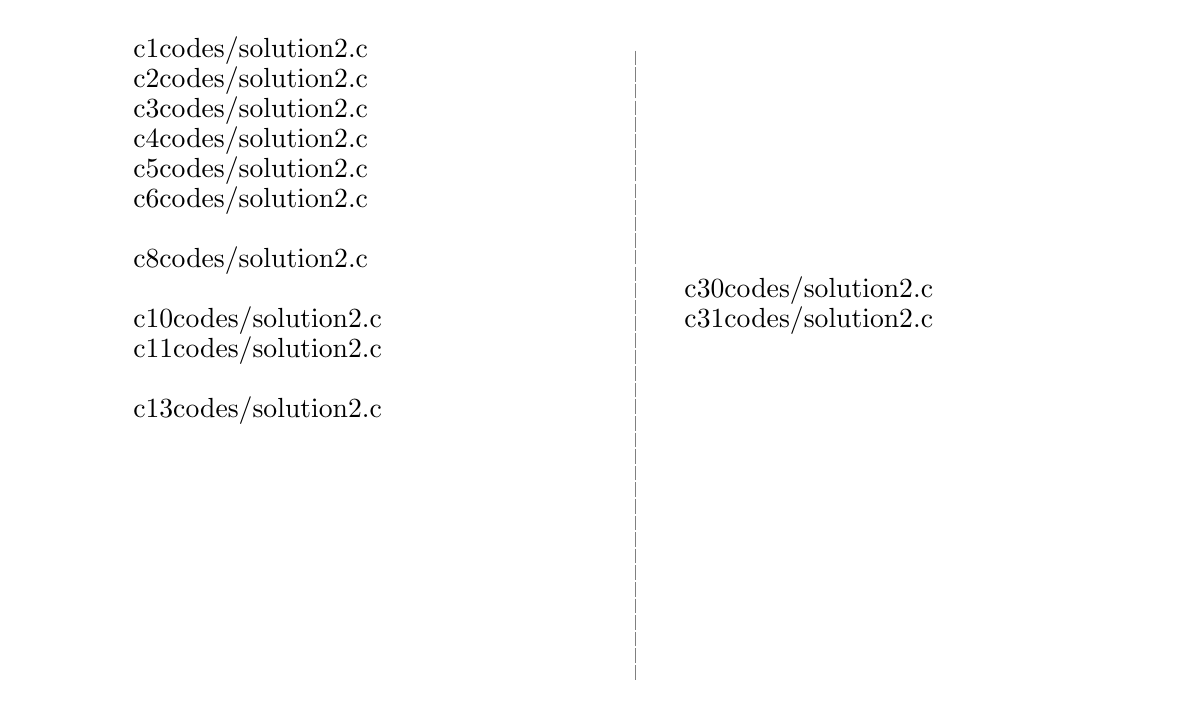
\begin{tikzpicture}
\node[draw,opacity=0] at (0, 0) {x};
\node[draw,opacity=0] at (14, 8) {x};

	\node[anchor=west] (line1) at (1.0, 8.0) { \inputline{c}{1}{codes/solution2.c} };

	\node[anchor=west] (line2) at (1.0, 7.62) { \inputline{c}{2}{codes/solution2.c} };

	\node[anchor=west] (line3) at (1.0, 7.24) { \inputline{c}{3}{codes/solution2.c} };

	\node[anchor=west] (line4) at (1.0, 6.86) { \inputline{c}{4}{codes/solution2.c} };

	\node[anchor=west] (line5) at (1.0, 6.48) { \inputline{c}{5}{codes/solution2.c} };

	\node[anchor=west] (line6) at (1.0, 6.1) { \inputline{c}{6}{codes/solution2.c} };


	\node[anchor=west] (line8) at (1.0, 5.33) { \inputline{c}{8}{codes/solution2.c} };


	\node[anchor=west] (line10) at (1.0, 4.57) { \inputline{c}{10}{codes/solution2.c} };

	\node[anchor=west] (line11) at (1.0, 4.19) { \inputline{c}{11}{codes/solution2.c} };


	\node[anchor=west] (line13) at (1.0, 3.43) { \inputline{c}{13}{codes/solution2.c} };










	\draw[color=gray,dashed] (7.5, 8) -- (7.5, 0) -- cycle;







	\node[anchor=west] (line30) at (8.0, 4.95) { \inputline{c}{30}{codes/solution2.c} };

	\node[anchor=west] (line31) at (8.0, 4.57) { \inputline{c}{31}{codes/solution2.c} };








\end{tikzpicture}
\end{frame}
\begin{frame}[plain,t]
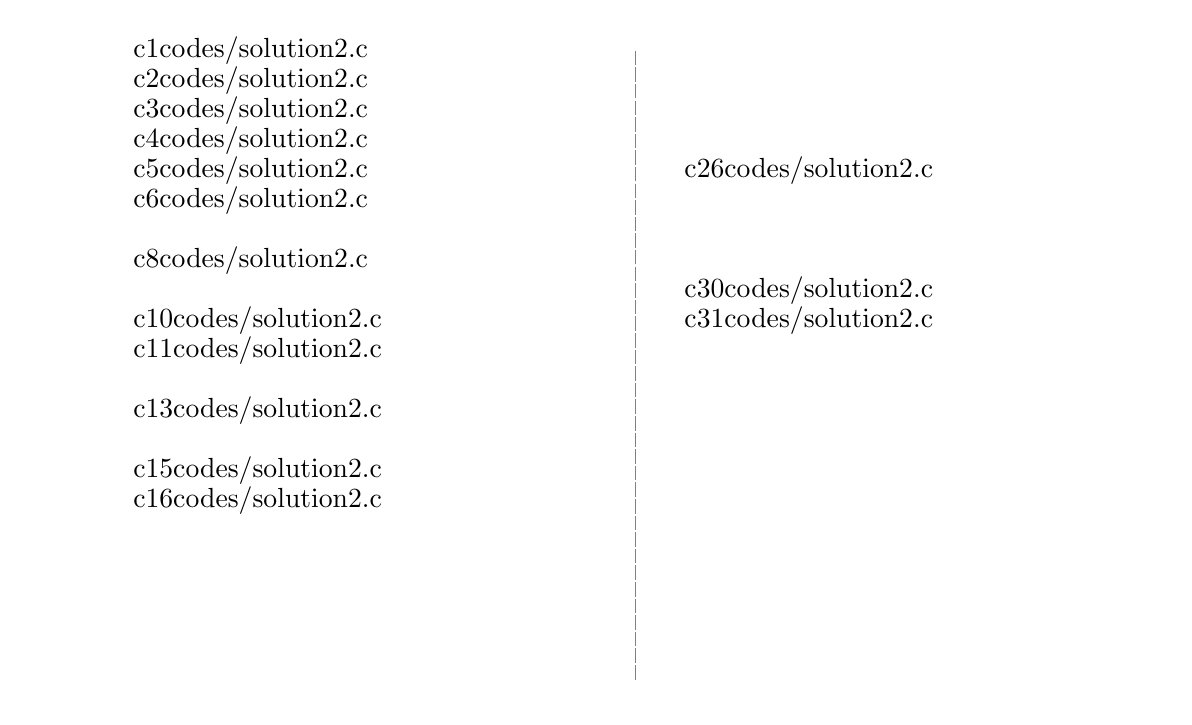
\begin{tikzpicture}
\node[draw,opacity=0] at (0, 0) {x};
\node[draw,opacity=0] at (14, 8) {x};

	\node[anchor=west] (line1) at (1.0, 8.0) { \inputline{c}{1}{codes/solution2.c} };

	\node[anchor=west] (line2) at (1.0, 7.62) { \inputline{c}{2}{codes/solution2.c} };

	\node[anchor=west] (line3) at (1.0, 7.24) { \inputline{c}{3}{codes/solution2.c} };

	\node[anchor=west] (line4) at (1.0, 6.86) { \inputline{c}{4}{codes/solution2.c} };

	\node[anchor=west] (line5) at (1.0, 6.48) { \inputline{c}{5}{codes/solution2.c} };

	\node[anchor=west] (line6) at (1.0, 6.1) { \inputline{c}{6}{codes/solution2.c} };


	\node[anchor=west] (line8) at (1.0, 5.33) { \inputline{c}{8}{codes/solution2.c} };


	\node[anchor=west] (line10) at (1.0, 4.57) { \inputline{c}{10}{codes/solution2.c} };

	\node[anchor=west] (line11) at (1.0, 4.19) { \inputline{c}{11}{codes/solution2.c} };


	\node[anchor=west] (line13) at (1.0, 3.43) { \inputline{c}{13}{codes/solution2.c} };


	\node[anchor=west] (line15) at (1.0, 2.67) { \inputline{c}{15}{codes/solution2.c} };

	\node[anchor=west] (line16) at (1.0, 2.29) { \inputline{c}{16}{codes/solution2.c} };







	\draw[color=gray,dashed] (7.5, 8) -- (7.5, 0) -- cycle;



	\node[anchor=west] (line26) at (8.0, 6.48) { \inputline{c}{26}{codes/solution2.c} };




	\node[anchor=west] (line30) at (8.0, 4.95) { \inputline{c}{30}{codes/solution2.c} };

	\node[anchor=west] (line31) at (8.0, 4.57) { \inputline{c}{31}{codes/solution2.c} };










\end{tikzpicture}
\end{frame}
\begin{frame}[plain,t]
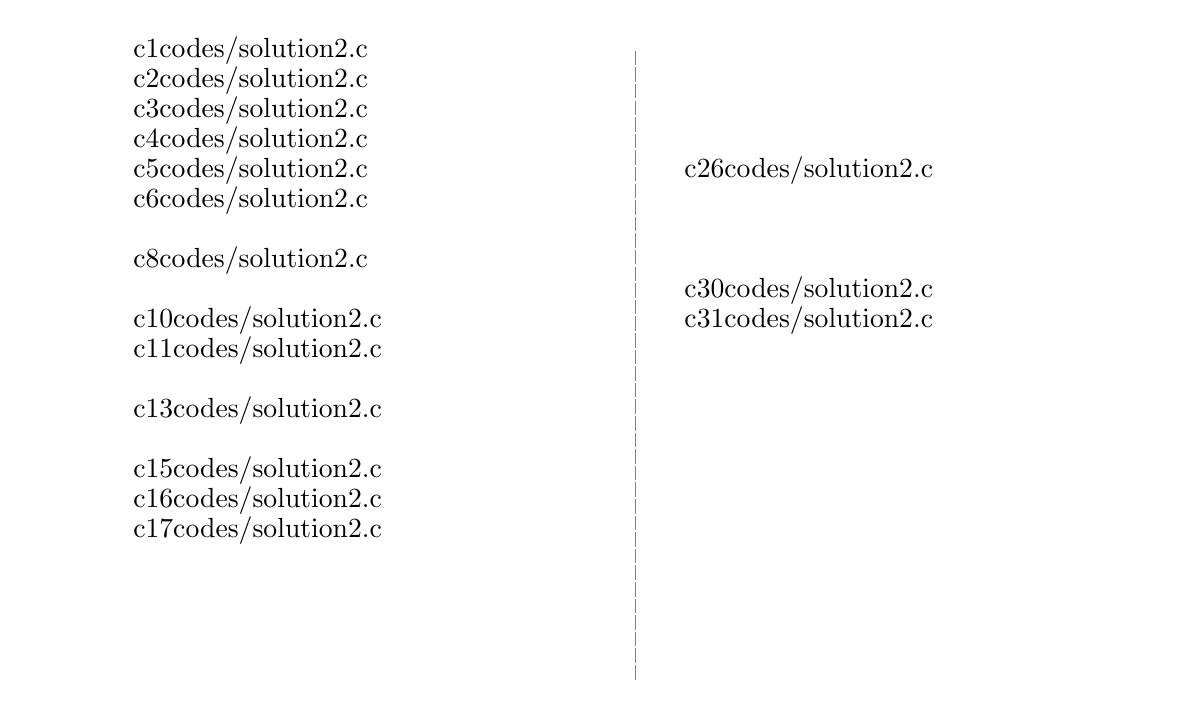
\begin{tikzpicture}
\node[draw,opacity=0] at (0, 0) {x};
\node[draw,opacity=0] at (14, 8) {x};

	\node[anchor=west] (line1) at (1.0, 8.0) { \inputline{c}{1}{codes/solution2.c} };

	\node[anchor=west] (line2) at (1.0, 7.62) { \inputline{c}{2}{codes/solution2.c} };

	\node[anchor=west] (line3) at (1.0, 7.24) { \inputline{c}{3}{codes/solution2.c} };

	\node[anchor=west] (line4) at (1.0, 6.86) { \inputline{c}{4}{codes/solution2.c} };

	\node[anchor=west] (line5) at (1.0, 6.48) { \inputline{c}{5}{codes/solution2.c} };

	\node[anchor=west] (line6) at (1.0, 6.1) { \inputline{c}{6}{codes/solution2.c} };


	\node[anchor=west] (line8) at (1.0, 5.33) { \inputline{c}{8}{codes/solution2.c} };


	\node[anchor=west] (line10) at (1.0, 4.57) { \inputline{c}{10}{codes/solution2.c} };

	\node[anchor=west] (line11) at (1.0, 4.19) { \inputline{c}{11}{codes/solution2.c} };


	\node[anchor=west] (line13) at (1.0, 3.43) { \inputline{c}{13}{codes/solution2.c} };


	\node[anchor=west] (line15) at (1.0, 2.67) { \inputline{c}{15}{codes/solution2.c} };

	\node[anchor=west] (line16) at (1.0, 2.29) { \inputline{c}{16}{codes/solution2.c} };

	\node[anchor=west] (line17) at (1.0, 1.9) { \inputline{c}{17}{codes/solution2.c} };






	\draw[color=gray,dashed] (7.5, 8) -- (7.5, 0) -- cycle;



	\node[anchor=west] (line26) at (8.0, 6.48) { \inputline{c}{26}{codes/solution2.c} };




	\node[anchor=west] (line30) at (8.0, 4.95) { \inputline{c}{30}{codes/solution2.c} };

	\node[anchor=west] (line31) at (8.0, 4.57) { \inputline{c}{31}{codes/solution2.c} };












\end{tikzpicture}
\end{frame}
\begin{frame}[plain,t]
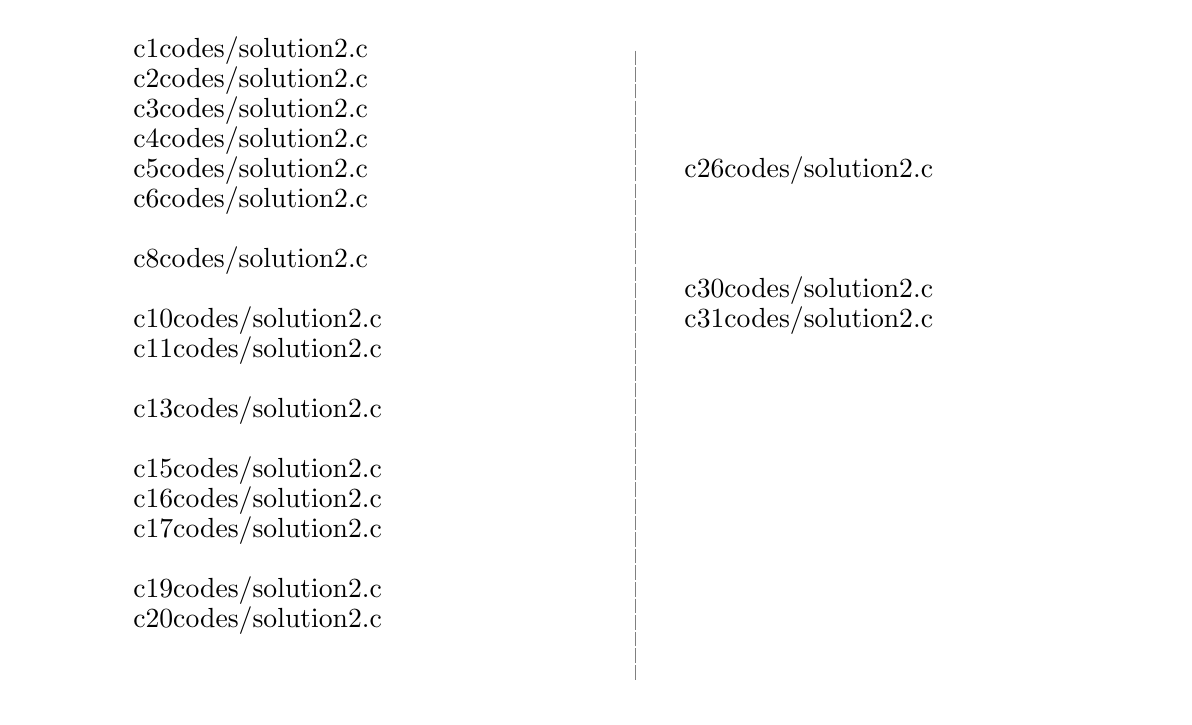
\begin{tikzpicture}
\node[draw,opacity=0] at (0, 0) {x};
\node[draw,opacity=0] at (14, 8) {x};

	\node[anchor=west] (line1) at (1.0, 8.0) { \inputline{c}{1}{codes/solution2.c} };

	\node[anchor=west] (line2) at (1.0, 7.62) { \inputline{c}{2}{codes/solution2.c} };

	\node[anchor=west] (line3) at (1.0, 7.24) { \inputline{c}{3}{codes/solution2.c} };

	\node[anchor=west] (line4) at (1.0, 6.86) { \inputline{c}{4}{codes/solution2.c} };

	\node[anchor=west] (line5) at (1.0, 6.48) { \inputline{c}{5}{codes/solution2.c} };

	\node[anchor=west] (line6) at (1.0, 6.1) { \inputline{c}{6}{codes/solution2.c} };


	\node[anchor=west] (line8) at (1.0, 5.33) { \inputline{c}{8}{codes/solution2.c} };


	\node[anchor=west] (line10) at (1.0, 4.57) { \inputline{c}{10}{codes/solution2.c} };

	\node[anchor=west] (line11) at (1.0, 4.19) { \inputline{c}{11}{codes/solution2.c} };


	\node[anchor=west] (line13) at (1.0, 3.43) { \inputline{c}{13}{codes/solution2.c} };


	\node[anchor=west] (line15) at (1.0, 2.67) { \inputline{c}{15}{codes/solution2.c} };

	\node[anchor=west] (line16) at (1.0, 2.29) { \inputline{c}{16}{codes/solution2.c} };

	\node[anchor=west] (line17) at (1.0, 1.9) { \inputline{c}{17}{codes/solution2.c} };


	\node[anchor=west] (line19) at (1.0, 1.14) { \inputline{c}{19}{codes/solution2.c} };

	\node[anchor=west] (line20) at (1.0, 0.76) { \inputline{c}{20}{codes/solution2.c} };



	\draw[color=gray,dashed] (7.5, 8) -- (7.5, 0) -- cycle;



	\node[anchor=west] (line26) at (8.0, 6.48) { \inputline{c}{26}{codes/solution2.c} };




	\node[anchor=west] (line30) at (8.0, 4.95) { \inputline{c}{30}{codes/solution2.c} };

	\node[anchor=west] (line31) at (8.0, 4.57) { \inputline{c}{31}{codes/solution2.c} };














\end{tikzpicture}
\end{frame}
\begin{frame}[plain,t]
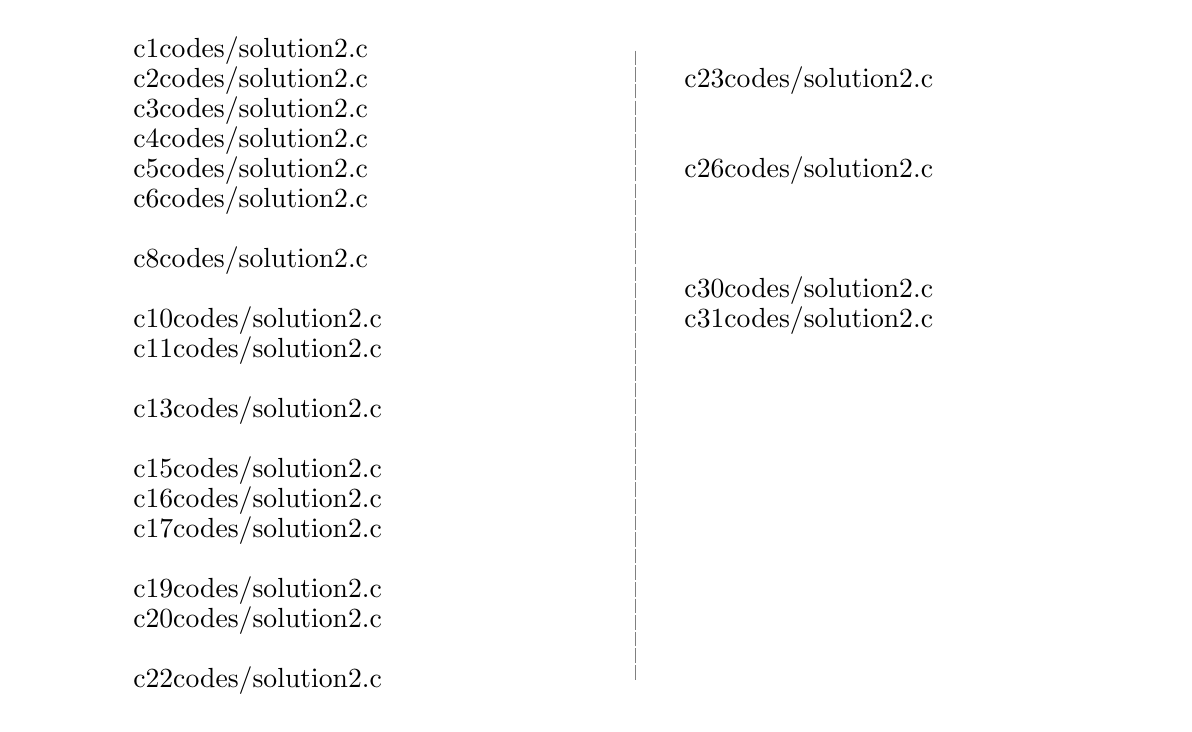
\begin{tikzpicture}
\node[draw,opacity=0] at (0, 0) {x};
\node[draw,opacity=0] at (14, 8) {x};

	\node[anchor=west] (line1) at (1.0, 8.0) { \inputline{c}{1}{codes/solution2.c} };

	\node[anchor=west] (line2) at (1.0, 7.62) { \inputline{c}{2}{codes/solution2.c} };

	\node[anchor=west] (line3) at (1.0, 7.24) { \inputline{c}{3}{codes/solution2.c} };

	\node[anchor=west] (line4) at (1.0, 6.86) { \inputline{c}{4}{codes/solution2.c} };

	\node[anchor=west] (line5) at (1.0, 6.48) { \inputline{c}{5}{codes/solution2.c} };

	\node[anchor=west] (line6) at (1.0, 6.1) { \inputline{c}{6}{codes/solution2.c} };


	\node[anchor=west] (line8) at (1.0, 5.33) { \inputline{c}{8}{codes/solution2.c} };


	\node[anchor=west] (line10) at (1.0, 4.57) { \inputline{c}{10}{codes/solution2.c} };

	\node[anchor=west] (line11) at (1.0, 4.19) { \inputline{c}{11}{codes/solution2.c} };


	\node[anchor=west] (line13) at (1.0, 3.43) { \inputline{c}{13}{codes/solution2.c} };


	\node[anchor=west] (line15) at (1.0, 2.67) { \inputline{c}{15}{codes/solution2.c} };

	\node[anchor=west] (line16) at (1.0, 2.29) { \inputline{c}{16}{codes/solution2.c} };

	\node[anchor=west] (line17) at (1.0, 1.9) { \inputline{c}{17}{codes/solution2.c} };


	\node[anchor=west] (line19) at (1.0, 1.14) { \inputline{c}{19}{codes/solution2.c} };

	\node[anchor=west] (line20) at (1.0, 0.76) { \inputline{c}{20}{codes/solution2.c} };


	\node[anchor=west] (line22) at (1.0, -0.0) { \inputline{c}{22}{codes/solution2.c} };

	\draw[color=gray,dashed] (7.5, 8) -- (7.5, 0) -- cycle;
	\node[anchor=west] (line23) at (8.0, 7.62) { \inputline{c}{23}{codes/solution2.c} };



	\node[anchor=west] (line26) at (8.0, 6.48) { \inputline{c}{26}{codes/solution2.c} };




	\node[anchor=west] (line30) at (8.0, 4.95) { \inputline{c}{30}{codes/solution2.c} };

	\node[anchor=west] (line31) at (8.0, 4.57) { \inputline{c}{31}{codes/solution2.c} };
















\end{tikzpicture}
\end{frame}
\begin{frame}[plain,t]
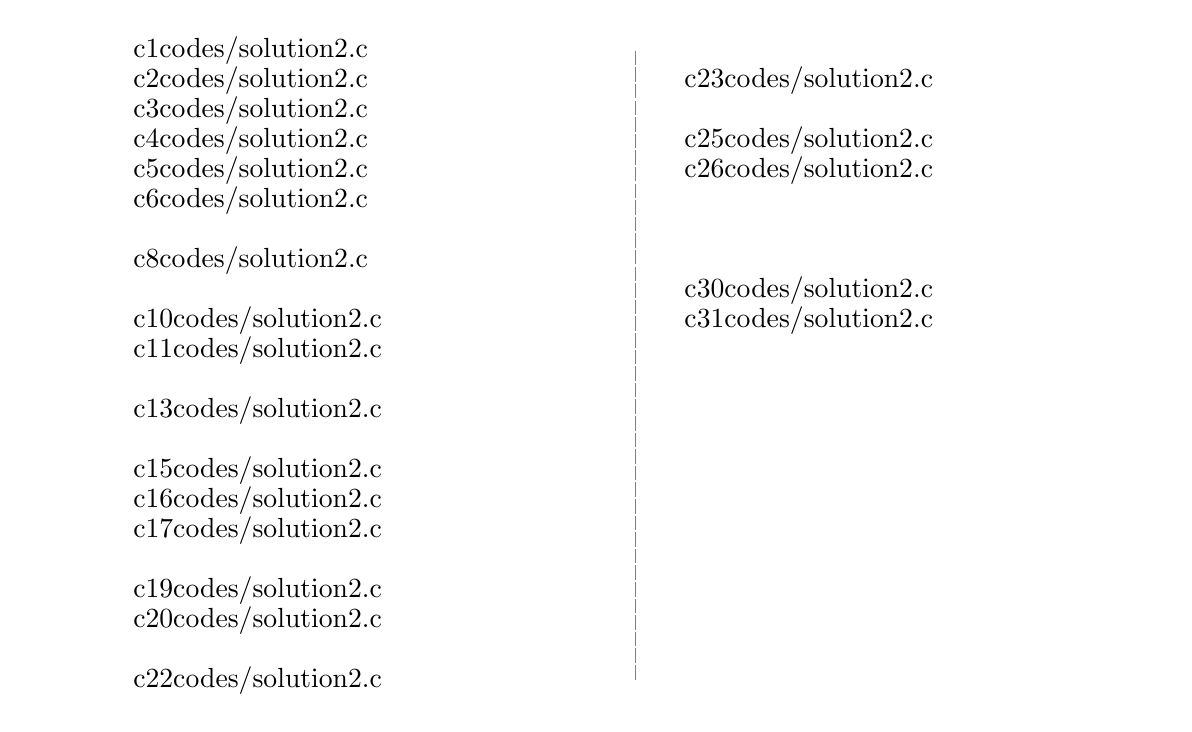
\begin{tikzpicture}
\node[draw,opacity=0] at (0, 0) {x};
\node[draw,opacity=0] at (14, 8) {x};

	\node[anchor=west] (line1) at (1.0, 8.0) { \inputline{c}{1}{codes/solution2.c} };

	\node[anchor=west] (line2) at (1.0, 7.62) { \inputline{c}{2}{codes/solution2.c} };

	\node[anchor=west] (line3) at (1.0, 7.24) { \inputline{c}{3}{codes/solution2.c} };

	\node[anchor=west] (line4) at (1.0, 6.86) { \inputline{c}{4}{codes/solution2.c} };

	\node[anchor=west] (line5) at (1.0, 6.48) { \inputline{c}{5}{codes/solution2.c} };

	\node[anchor=west] (line6) at (1.0, 6.1) { \inputline{c}{6}{codes/solution2.c} };


	\node[anchor=west] (line8) at (1.0, 5.33) { \inputline{c}{8}{codes/solution2.c} };


	\node[anchor=west] (line10) at (1.0, 4.57) { \inputline{c}{10}{codes/solution2.c} };

	\node[anchor=west] (line11) at (1.0, 4.19) { \inputline{c}{11}{codes/solution2.c} };


	\node[anchor=west] (line13) at (1.0, 3.43) { \inputline{c}{13}{codes/solution2.c} };


	\node[anchor=west] (line15) at (1.0, 2.67) { \inputline{c}{15}{codes/solution2.c} };

	\node[anchor=west] (line16) at (1.0, 2.29) { \inputline{c}{16}{codes/solution2.c} };

	\node[anchor=west] (line17) at (1.0, 1.9) { \inputline{c}{17}{codes/solution2.c} };


	\node[anchor=west] (line19) at (1.0, 1.14) { \inputline{c}{19}{codes/solution2.c} };

	\node[anchor=west] (line20) at (1.0, 0.76) { \inputline{c}{20}{codes/solution2.c} };


	\node[anchor=west] (line22) at (1.0, -0.0) { \inputline{c}{22}{codes/solution2.c} };

	\draw[color=gray,dashed] (7.5, 8) -- (7.5, 0) -- cycle;
	\node[anchor=west] (line23) at (8.0, 7.62) { \inputline{c}{23}{codes/solution2.c} };


	\node[anchor=west] (line25) at (8.0, 6.86) { \inputline{c}{25}{codes/solution2.c} };

	\node[anchor=west] (line26) at (8.0, 6.48) { \inputline{c}{26}{codes/solution2.c} };




	\node[anchor=west] (line30) at (8.0, 4.95) { \inputline{c}{30}{codes/solution2.c} };

	\node[anchor=west] (line31) at (8.0, 4.57) { \inputline{c}{31}{codes/solution2.c} };


















\end{tikzpicture}
\end{frame}
\begin{frame}[plain,t]
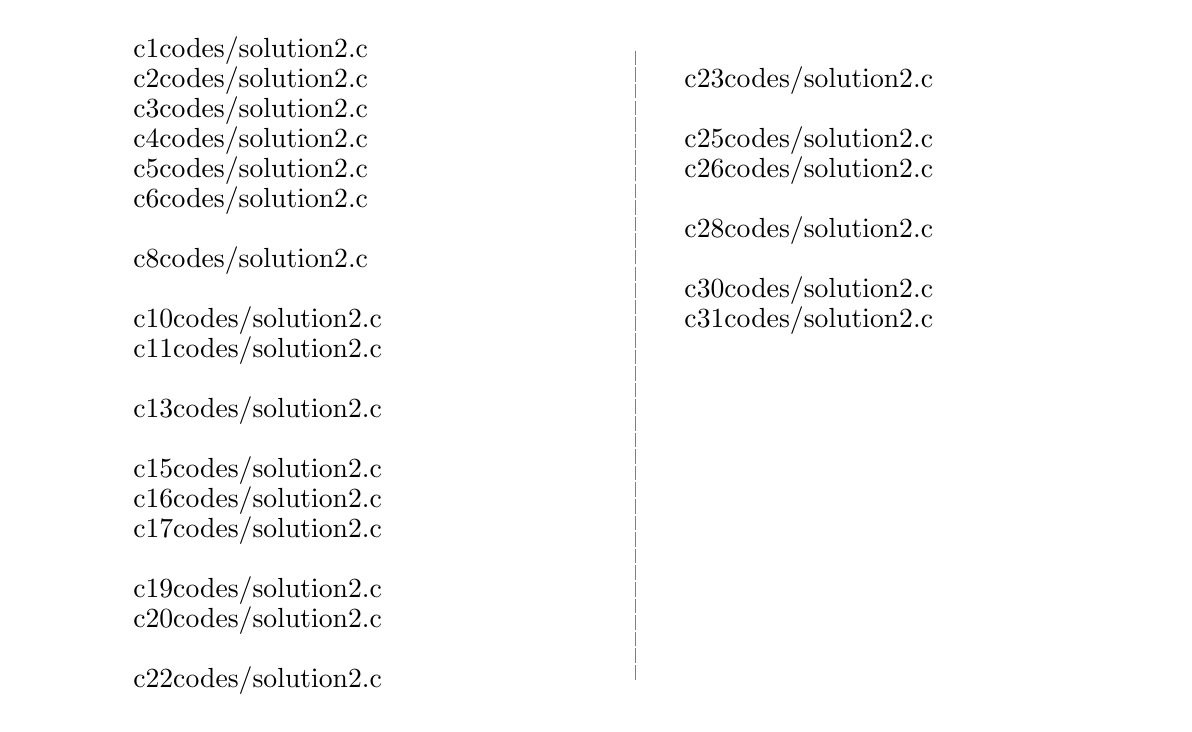
\begin{tikzpicture}
\node[draw,opacity=0] at (0, 0) {x};
\node[draw,opacity=0] at (14, 8) {x};

	\node[anchor=west] (line1) at (1.0, 8.0) { \inputline{c}{1}{codes/solution2.c} };

	\node[anchor=west] (line2) at (1.0, 7.62) { \inputline{c}{2}{codes/solution2.c} };

	\node[anchor=west] (line3) at (1.0, 7.24) { \inputline{c}{3}{codes/solution2.c} };

	\node[anchor=west] (line4) at (1.0, 6.86) { \inputline{c}{4}{codes/solution2.c} };

	\node[anchor=west] (line5) at (1.0, 6.48) { \inputline{c}{5}{codes/solution2.c} };

	\node[anchor=west] (line6) at (1.0, 6.1) { \inputline{c}{6}{codes/solution2.c} };


	\node[anchor=west] (line8) at (1.0, 5.33) { \inputline{c}{8}{codes/solution2.c} };


	\node[anchor=west] (line10) at (1.0, 4.57) { \inputline{c}{10}{codes/solution2.c} };

	\node[anchor=west] (line11) at (1.0, 4.19) { \inputline{c}{11}{codes/solution2.c} };


	\node[anchor=west] (line13) at (1.0, 3.43) { \inputline{c}{13}{codes/solution2.c} };


	\node[anchor=west] (line15) at (1.0, 2.67) { \inputline{c}{15}{codes/solution2.c} };

	\node[anchor=west] (line16) at (1.0, 2.29) { \inputline{c}{16}{codes/solution2.c} };

	\node[anchor=west] (line17) at (1.0, 1.9) { \inputline{c}{17}{codes/solution2.c} };


	\node[anchor=west] (line19) at (1.0, 1.14) { \inputline{c}{19}{codes/solution2.c} };

	\node[anchor=west] (line20) at (1.0, 0.76) { \inputline{c}{20}{codes/solution2.c} };


	\node[anchor=west] (line22) at (1.0, -0.0) { \inputline{c}{22}{codes/solution2.c} };

	\draw[color=gray,dashed] (7.5, 8) -- (7.5, 0) -- cycle;
	\node[anchor=west] (line23) at (8.0, 7.62) { \inputline{c}{23}{codes/solution2.c} };


	\node[anchor=west] (line25) at (8.0, 6.86) { \inputline{c}{25}{codes/solution2.c} };

	\node[anchor=west] (line26) at (8.0, 6.48) { \inputline{c}{26}{codes/solution2.c} };


	\node[anchor=west] (line28) at (8.0, 5.71) { \inputline{c}{28}{codes/solution2.c} };


	\node[anchor=west] (line30) at (8.0, 4.95) { \inputline{c}{30}{codes/solution2.c} };

	\node[anchor=west] (line31) at (8.0, 4.57) { \inputline{c}{31}{codes/solution2.c} };




















\end{tikzpicture}
\end{frame}
\end{document}
